\documentclass{fast_latex}
% yay! We can use any kind of funky diacritic:
\usepackage[utf8]{inputenc}

\usepackage{lastpage}
\usepackage{setspace}
\usepackage[pdfborder={0 0 0}]{hyperref}        % turn on when latex is used (not miktec)
\usepackage{url} % LEO: urls \url{}
\usepackage{verbatim} % code and comment
\usepackage{longtable}
\usepackage{xspace}   % whitespace after a macro if no punctuation after the macro
\usepackage{lipsum}
\usepackage{multirow}
\usepackage{colortbl}
\usepackage{array}
\usepackage{textcomp} %vertical apostrophe
\usepackage{listings} %source code listings
\usepackage{amssymb} %math symbols
\usepackage{graphicx} %image placement
\usepackage{supertabular}

\usepackage{amsmath}
\usepackage{pgf} %graph plot
\usepackage{tikz}
\usetikzlibrary{plotmarks}

\usepackage{listings} %source code listings
\usepackage{paralist}
\usepackage{booktabs}

\parindent0pt

\newcommand\deliverableNumber{D2.4.3}
\newcommand\deliverableTitle{Mediation amongst ontologies: Application to the FAST platform}
\newcommand\deliverableTitleShort{Mediation amongst ontologies}
\newcommand\workpackageNumber{2}
\newcommand\workpackageTitle{Definition of Conceptual Model}
\newcommand\authorOne{Oszkar Ambrus (NUIG)}
\newcommand\authorTwo{Knud M\"{o}ller (NUIG)}
\newcommand\authorThree{Albert Z\"{u}ndorf (UniKassel)}
\newcommand\authorFour{J\"{o}rn Friedrich Dreyer (UniKassel)}
\newcommand\authorFive{Sebasti\'{a}n Ortega (UPM)}
\newtheorem{example}{\emph{Example}}

\begin{document}
% explicit hyphenations
\hyphenation{RDF-Re-po-si-to-ry}
\hyphenation{name-space}
\hyphenation{So-cket-A-dap-ter}

%\fontfamily{tahoma}\selectfont
\def\note#1{\marginpar{\footnotesize#1}} % use this to show the notes in the document
%\def\note#1{} % use this to hide the notes



%%%%%%%%%%%%%%%%%%%%%%%%%%%%%%%%%%%%%%%%%%%%%%%%%%%%%%%%%%%%%%%%%%%%%%%%%%%%%%%%
% TITLE PAGES 
%%%%%%%%%%%%%%%%%%%%%%%%%%%%%%%%%%%%%%%%%%%%%%%%%%%%%%%%%%%%%%%%%%%%%%%%%%%%%%%%
\thispagestyle{empty}

%\pagenumbering{roman}
\pagenumbering{arabic}

\begin{flushright}
    
\includegraphics[width=3cm]{images/FP7_logo.png}
\end{flushright}

\vspace{1cm}

%\begin{minipage}[p]{15cm}
    \begin{center}
        
\includegraphics{images/FAST_logo}\\
        \vspace{1cm}
        {\LARGE{\sffamily \emph{FAST AND ADVANCED STORYBOARD TOOLS}}}\\
        \vspace{0.5cm}
        {\LARGE \sffamily \emph{FP7-ICT-2007-1-216048}}\\
        \vspace{0.5cm}
        {\LARGE \sffamily \emph{http://fast.morfeo-project.eu}}\\
        \vspace{4cm}
        {\LARGE \sffamily \textbf{Deliverable \deliverableNumber}}\\
        \vspace{0.5cm}
        {\LARGE \sffamily \textbf{\deliverableTitle}}\\
        \vspace{2cm}
        {\large \sffamily \authorOne} \\
        {\large \sffamily \authorTwo} \\
        {\large \sffamily \authorThree} \\
        {\large \sffamily \authorFour} \\
        {\large \sffamily \authorFive} \\
        \vspace{0.5cm}
        \vfill
        {\large \sffamily Date: 27/02/2011}\\
        \vspace{1cm}
        {\sffamily FAST is partially funded by the E.C. (grant code: FP7-ICT-2007-1-216048).}
        
    \end{center}
%\end{minipage}


\clearpage
%%%%%%%%%%%%%%
% NEXT PAGES %
%%%%%%%%%%%%%%
\pagestyle{scrheadings}

\lohead{
\includegraphics[width=4cm]{images/FAST_logo_transparent}}
%\cohead{\small\textcolor{fast@lightgrey}{\deliverableTitle}}
%\rohead{\small{\today}}
%\lofoot{\small\textcolor{fast@lightgrey}{Task Force Ontologies}}
\cofoot{\small{FAST $\bullet$ 216048 $\bullet$ \deliverableTitleShort\ $\bullet$ Page \thepage\ of \pageref{LastPage}}}
%\rofoot{\small{}}
%\rofoot{\small{\thepage}}

\newpage
%
%\section*{Authors}
%\authorOne \\
%%\authorTwo \\
%%\authorThree\\
%%\authorFour\\
%
%
%\vfill
%%\section*{Project Co-ordinator}
%%\hspace*{-2,5cm}\begin{minipage}[p]{14cm}
%%Dr. Ansgar Bernardi \\
%%German Research Center for Artificial Intelligence (DFKI) GmbH \\
%%Trippstadter Strasse 122 \\
%%D 67663 Kaiserslautern \\
%%Germany \\
%%Email: bernardi@dfki.uni-kl.de, phone: +49 631 205 3582, fax: +49 631 205 4910 \\
%%\end{minipage}
%
%
%\section*{Partners}
%Telef\'onica Investigaci\'on y Desarrollo (Telef\'onica I+D), Spain \\
%National University of Ireland, Galway (NUIG), Republic of Ireland \\
%Kassel University, Germany \\
%Cyntelix Corporation, Republic of Ireland \\
%SAP AG, Germany \\
%Universidad Polit\'ecnica de Madrid (UPM), Spain
%
%
%\vspace{0.3cm}
%\begin{footnotesize}
%Copyright: FAST Consortium 2009\\
%\end{footnotesize}

%\clearpage


\section*{Version History}

\begin{small}
\begin{tabular}{|l|l|l|p{7.5cm}|}
\hline
\rowcolor{fast@lightgrey}\textcolor{white}{\textbf{Rev. No.}} &
                            \textcolor{white}{\textbf{Date}} &
                            \textcolor{white}{\textbf{Author (Partner)}} &
                            \textcolor{white}{\textbf{Change description}}\\ \hline
% 0.1 & 09.05.2009 & \authorOne & Initial content \\ \hline
% 0.4 & 30.11.2009 & \authorOne & Sections 2 and 3 \\ \hline
% 0.5 & 07.01.2010 & \authorOne & New structure, Section 4 and 5 \\ \hline
% 0.7 & 03.02.2010 & \authorTwo & Section 3.5, 3.6, updated Section 5  \\ \hline
% 0.8 & 03.02.2010 & \authorOne & Integration and preliminary finalization  \\ \hline
% 0.9 & 03.02.2010 & NUIG, UniKassel & Corrections  \\ \hline
% 1.0 & 03.02.2010 & \authorOne & Integration and finalization  \\ \hline
%0.2 & 19.02.2009 & Oszkar Ambrus (NUIG) & content moved from wiki after internal review \\ \hline
%0.1 & 07.01.2009 & Oszkar Ambrus (NUIG) & final version ready for external review \\ \hline
1.0 & 27.02.2009 & \authorOne & final version (D2.4.1) ready for external review \\ \hline
2.0 & 27.02.2010 & \authorOne & final version (D2.4.2) ready for external review \\ \hline
3.0 & 27.02.2011 & \authorTwo & final version (D2.4.3) ready for external review \\ \hline
\end{tabular}
\end{small}

\color{black}

\vfill
%{\bf Explanations of abbreviations on front page}\\
%\\
%%Nature \\
%R: Report \\
%P: Prototype \\
%R/P: Report and Prototype \\
%O: Other \\
% \\
%Dissemination level \\
%PU: Public \\
%PP: Restricted to other FP6 participants \\
%RE: Restricted to specified group \\
%CO: Confidential, only for NEPOMUK partners \\

\newpage

%%%%%%%%%%%%%%%%%%%%%
% Executive Summary %
%%%%%%%%%%%%%%%%%%%%%

\clearpage

\section*{Executive Summary}
\doublespacing
Ontology mediation is a critical problem in heterogeneous environments, since inter-operating services and agents often use different
ontologies, and the differences between them need to be determined and overcome to allow for a seamless data exchange between these parties.
This is a difficult task, with which web-based agents must cope. 

In D2.4.1 we reviewed current work and literature, discussing the main areas of the topic, that is the core problem of ontology mediation, the types of mismatches that occur between ontologies, and the three main ontology mediation approaches, namely (1) the representation of correspondences between ontologies, (2) the (semi-)automatic process of discovering these correspondences and (3) creation of a new ontology from the source ontologies. 

Based on the theoretical foundations laid down in D2.4.1 we present our approach to integrating ontology matching into the FAST platform. We present the roles related to ontology matching in FAST, and the way ontology matching is achieved within each one of those roles.

\newpage

%%%%%%%%%%%%%%%%%%%%%
% Document Summary %
%%%%%%%%%%%%%%%%%%%%%

\clearpage

\section*{Document Summary}
% double spacing from here on:
\singlespacing
\begin{small}

\begin{tabular}
    %{| >{\columncolor{fast@lightgrey}}p{3.25cm}|p{6cm}|p{2cm}|p{2cm}|}
    {| >{\columncolor{fast@lightgrey}}p{3.25cm}|p{6cm}|p{2cm}|p{2cm}|}
    \hline
    \textcolor{white}{\textbf{Code}} & {FP7-ICT-2007-1-216048} & {\textbf{Acronym}} & {FAST}\\ \hline
    \textcolor{white}{\textbf{Full title}} & \multicolumn{3}{l|}{Fast and Advanced Storyboard Tools}\\ \hline
    \textcolor{white}{\textbf{URL}} & \multicolumn{3}{l|}{\url{http://fast.morfeo-project.eu}}\\ \hline
    \textcolor{white}{\textbf{Project officer}} & \multicolumn{3}{l|}{Annalisa Bogliolo}\\ \hline
\end{tabular}

\vspace{0.5cm}

\begin{tabular}
    {| >{\columncolor{fast@lightgrey}}p{3.25cm}|p{1.25cm}|p{1cm}|p{1cm}|p{6.32cm}|}
    \hline
    \textcolor{white}{\textbf{Deliverable}} & {\textbf{Number}} & {\deliverableNumber} & {\textbf{Name}} & {\deliverableTitle}\\ \hline
    \textcolor{white}{\textbf{Work package}} & {\textbf{Number}} & {\workpackageNumber} & {\textbf{Name}} & {\workpackageTitle}\\ \hline
\end{tabular}

\vspace{0.5cm}

\begin{tabular}
    {| >{\columncolor{fast@lightgrey}}p{3.25cm}|p{1.4cm}|p{3.28cm}|p{1.6cm}|p{3.29cm}|}
    \hline
    \textcolor{white}{\textbf{Delivery data}} & {\textbf{Due date}} & {28/02/2011} & {\textbf{Submitted}} & {27/02/2011}\\ \hline
    \textcolor{white}{\textbf{Status}} & \multicolumn{2}{l|}{} & \multicolumn{2}{l|}{final}\\ \hline
    \textcolor{white}{\textbf{Dissemination Level}} & \multicolumn{4}{l|}{Public $\boxtimes$ / Consortium $\square$}\\ \hline
    \textcolor{white}{\textbf{Short description of contents}} & \multicolumn{4}{p{10.85cm}|}{D2.4.3 is the third iteration of the FAST ontology matching approach. The first iteration contained a general overview of the literature regarding ontology mediation, paving the way for further analysis of the scenarios arising in FAST that require ontology mediation. Based on that general overview, this current iteration presents the approach to implement ontology matching within FAST. We present the different roles within the platform, tasks and challenges related to them, and the way ontology matching is integrated within each role.}\\ \hline
    \textcolor{white}{\textbf{Authors}} & \multicolumn{4}{p{10.85cm}|}{\authorOne,  \authorTwo, \authorThree, \authorFour, \authorFive}\\
%   {} & \multicolumn{4}{l|}{}\\ 
%   {} & \multicolumn{4}{l|}{}\\ 
%   {} & \multicolumn{4}{l|}{}\\
    \hline
    \textcolor{white}{\textbf{Deliverable Owner}} & \multicolumn{2}{l|}{\authorOne} & \textbf{email} & {knud.moeller@deri.org} \\ \cline{4-5}
    \textcolor{white}{\textbf{(Partner)}} & \multicolumn{2}{l|}{} & \textbf{phone} & {+353 91 495112} \\ \hline
    \textcolor{white}{\textbf{Keywords}} & \multicolumn{4}{p{10.85cm}|}{FAST, ontology mediation, ontology matching, ontology alignment}\\ \hline
\end{tabular}
\end{small}
\newpage

%%%%%%%%%%%%%%%%%%%%%
% TABLE OF CONTENTS %
%%%%%%%%%%%%%%%%%%%%%
\doublespacing
\setcounter{tocdepth}{3}
\tableofcontents
\clearpage
\section*{Lists of Tables and Figures}
\listoftables
\listoffigures
\cleardoublepage
%\pagenumbering{arabic}

%%%%%%%%%%%%%%%%%%%%%%%%%
% BEGINNING OF SECTIONS %
%%%%%%%%%%%%%%%%%%%%%%%%%
\clearpage
\rofoot{\small{Page \thepage\ of \pageref{LastPage}}}


\section{Introduction} %%%%%%%%%%%%%%%%%%%%%%%%%%%%%%%%
\label{sec:intro}
\subsection{Goal and Scope}
FAST is a visual programming platform allowing non-technical end users to build situational mashups, employing various underlying services and generating new ones. Resources in FAST are described semantically using different ontologies and vocabularies, and can therefore be combined to what we can call ``intelligent gadgets'', that rely on semantically enriched building blocks. In the services used within the FAST environment, the ontologies involved in the creation of gadgets and building blocks come from different parties. These ontologies, though different, will sometimes cover the same domain, making ontology matching necessary as the means to reconcile differences in the various conceptualisations.

We aim to integrate a form of ontology matching into the FAST platform to allow for discrepant systems to intercommunicate.  We try to find a solution to these differences which range from simple naming differences to more complex data heterogeneity, behavioural differences, discrepant paradigms and other disparities. The reconciliation of these differences is called ontology matching (often mentioned in the specialised literature as ontology mediation, or ontology alignment, thus we will sometimes use these terms as well). 

\subsubsection{Changes from Previous Version}

The following changes have been made with respect to the previous version of this deliverable, D2.4.2.~\cite{ambrus2010mediation}. A history of previous changes is kept in App.~\ref{sec:old_changes}.

\begin{itemize}
	\item In response to the previous review, we have extended and improved the text in order to better position ontology matching in FAST throughout the document.
	\item The previous D2.4.2 introduced the \emph{fact transformation tool}. At the time, this tool was an early stand-alone prototype. In the meantime, the fact tool has been properly integrated with the FAST tool chain. These improvements are reflected in both text and screenshots in Sects.~\ref{sec:fact_tool} and \ref{sec:creating_the_operator}. New content has been added to show how the output of the tool is used in screen development.
	\item The document as a whole has been revised, and minor changes (mostly, spelling, grammar and small updates to reflect latest developments) have been made throughout the deliverable.
\end{itemize}


\subsection{Structure of the Document}
This document describes the approach of integrating ontology matching into the FAST environment. Sect.~\ref{sec:overview} gives the big picture of ontology matching in fast, which the remaining three sections expand. Thus, Sect.~\ref{sec:ontologyengineering} describes a tool to automatically discover alignments, a scenario and example ontologies to demonstrate the capabilities of the tool, and the testing procedure with the results. The remaining part of the section deals with a tool to define the discovered mapping rules in a way that is consistent with other similar tasks within the FAST platform, and describes the way in which matching operators are stored within the Semantic Catalogue. Sect.~\ref{sec:gadgetbuilding} shortly describes the way the matching operator is used when composing screenflows and Sect.~\ref{sec:runtime} describes how the matching operator and the defined rules are converted and used in the final, deployed gadget.

%Describe the rest.
The Appendix contains the first iteration of this document, D2.4.1, laying down the theoretical foundations of ontology matching. We discuss ontologies in general in App.~\ref{sec:ontologies}, present the ontology mediation problem in App.~\ref{sec:mediationproblem} , discuss the types  of mismatches between ontologies in App.~\ref{sec:ontologymismatches} and detail the main approaches to ontology mediation in App.~\ref{sec:mediationapproaches}.

\subsection{Overall Approach for WP2 and relation to other Work Packages and Deliverables.}
Ontology matching will play an important role for the integration of different underlying resources in the user-built gadgets. 
We present our initial research in the implementation of ontology matching in this second iteration of D2.4, after having laid the theoretical ground work of ontology matching in the first iteration. The final version of the deliverable (i.e., D2.4.3) will complete the implementation of ontology mediation within the FAST platform. 

Parts of this work rely on the results of D4.3.2, where a service wrapper tool is described, that will be modified to be used in matching ontologies.

%\pagebreak
%\part{Implementing Ontology Matching within the FAST Platform}
%\label{part:d2.4.2}

%!TEX root = fast_d2_4_3_mediation.tex

\lstset{
captionpos=b, 
extendedchars=true,
basicstyle=\scriptsize \sffamily, 
stringstyle=\bfseries,
frame=single,
frameround=tttt,
showstringspaces=false,
breaklines=true,
}

\lstdefinelanguage{turtle} 
{morekeywords={@prefix, a}, 
sensitive=false, 
morecomment=[l]{\#}, 
morestring=[b]",
}

\section{Overview}
\label{sec:overview}

In this section, we introduce some general terminology and definitions regarding ontology matching, as well as positioning ontology matching in FAST in terms of user roles.

\subsection{Ontology Matching}
\label{mediation}

FAST uses ontologies to conceptualise resources and data used by the different components.
Ontologies embody the fundamental vehicle for conceptualising data on semantic systems; they describe the context and semantic background of data that should be known to all agents using it~\cite{gruber93towards}.
However, different ontologies are often used to describe the same domain or cover the same scenario. This is also true for FAST, where gadget building blocks can originate from different providers, who might use different ontologies to describe them. To ensure interoperability, the task of ontology matching is therefore important in FAST.

Given two ontologies $O$ and $O'$ that need to be mapped to each other, we adopt the definition given in~\cite{shvaiko2005schema_based}: an ontology mapping element is a 5-tuple $<id, e, e', n, R>$, where 
%\begin{inparaenum}[(i)]
$id$ is a unique identifier, identifying the
mapping element, 
$e$ and $e'$ are entities (formulas, terms, classes, individuals) of the first and second ontology, respectively, 
$n$ is a confidence measure holding the correspondence value between $e$ and
$e'$, 
$R$ is the correspondence relation holding between $e$ and $e'$ (e.g., \texttt{equivalence (=)}, \texttt{more general($\sqsupseteq$)} or \texttt{disjointness($\perp$)}).
%; \texttt{overlapping($\sqcap$)}. 
%\end{inparaenum}
The alignment operation determines the mapping $M'$ for a pair of ontologies $O$ and $O'$. The alignment process can be extended by parameters, such as an input mapping, weights and thresholds and other external resources (dictionaries, thesauri, etc.). Different levels of mappings are defined:

\begin{inparaenum}[(a)]
    \item A \textit{level 0} mapping~\cite{euzenat2004api} is a set of the above mapping elements, when the entities are discreet (defined by URIs). E.g., consider the ontology $O1$ with a class \texttt{Person}, and another ontology $O2$ with a class \texttt{Human}. For this case a matching algorithm  could return the mapping element $< id_{11}, Person, Human, 0.67, = >$, meaning that the \texttt{Person} class from the first ontology is found to be equivalent to the \texttt{Human} class in the second one with a confidence measure of \texttt{0.67}.
    \item A \textit{level 1} mapping is a slight refinement of level 0, replacing pairs of elements with pairs of sets of elements.
    \item A \textit{level 2} mapping can be more complex and defines correspondences in first order logic. It uses the ontology mapping language described in~\cite{scharffe2005language}. It can describe complex correspondences, such as the one detailed in Sect.~\ref{sub:manual_mapping}.
\end{inparaenum}
% :
% 
% \begin{equation*} \label{eq}
% \forall{x,z} grandparent(x,z) \Longrightarrow \exists{y}; parent(x,y) \wedge parent(y,z)
% \end{equation*}
 

\subsection{Ontology Matching in FAST}
\label{ominfast}

As detailed in \cite{hoyer2009fast}, the gadget life cycle in FAST has several phases and roles associated. Here, we list the ones relevant for the ontology matching tasks, in decreasing order of the measure in which knowledge about ontologies is required. Note that several roles can be played by the same actor.
\begin{enumerate}[(i)]
    \item The \textit{ontology engineer} creates the ontologies used to annotate services and data. This role also includes the process of ontology matching, either automated or manually, determining if the alignment is feasible and creating so-called \emph{matching operator} building blocks, which are basic elements of the FAST gadget building. The \textit{resource developer} then uses these ontologies to annotate resources created in FAST, which resources will be used by the \textit{screen developer}, who will also specify the resource type at the pre- and postconditions of a screen. These three roles are the most critical in FAST with respect to ontology matching, and topics relevant to these roles will be discussed in detail in Sect.~\ref{sec:ontologyengineering}.
    \item Ontology matching is needed by the \textit{gadget developer} at the design-time of a screen-flow (gadget). Gadget developers use the GVS (Gadget Visual Storyboard) for building gadgets, where they can use the matching operators to combine screens having input and output conditions specifying resources annotated with different ontologies. No actual matching needs to be performed in this phase, but rather the possibility of matching needs to be determined (i.e., \emph{can} two screens A and B be combined?).
%the FAST user interface determines if two resources can be combined or not (see Figure \ref{fig:screens} for a conceptual example of resources that can not be combined).
Section~\ref{sec:gadgetbuilding} outlines how the gadget developer if affected by ontology matching.
    %\item The \emph{gadget developer} combines screens to screen-flows and gadgets, and only uses ontology matching implicitly.
    \item The \textit{end-user} uses the final deployed gadget at run-time, but is unaware of the underlying resources and ontologies or the matching process. Only at run-time the actual mapping of instance data has to be performed.
This aspect of ontology matching is briefly discussed in Sect.~\ref{sec:runtime}.
\end{enumerate}


\section{Ontology Engineering Phase}
\label{sec:ontologyengineering}

In the FAST lifecycle, the ontology engineering phase is the most relevant for the topic of this deliverable. Relevant roles are the ontology engineer, who performs the main work in this phase, as well as the the resource developer and the screen developer, who are directly affected.

In this section, we present a number of tools that can be used to help the ontology engineer in creating mapping rules to mediate between different conceptualisations. Some ontologies relevant for an e-commerce use case are introduced, and their automatic mapping is evaluated using one of the tools. The evaluation shows that automatic mapping is feasible only in certain cases, while other cases require a manual approach. The section concludes with the presentation of a tool developed in FAST to facilitate the use of (either automatically or manually created) mapping rules within the FAST tool chain.

\subsection{Alignment Tool}
\label{alignmenttool}

An \emph{ontology mapping} is a declarative specification of the semantic overlap between two ontologies~\cite{debruin2005wsml}. It is the result of the \emph{ontology alignment process}. This mapping is represented as a set of axioms in a \emph{mapping language}. The mapping process has three main phases:
\begin{inparaenum}[(1)]
    \item discovering the mapping (alignment phase), 
    \item representing the mapping and 
    \item exploiting the mapping.
\end{inparaenum}  

To accomplish this we need a tool to assist the ontology engineer in the ontology mapping process.
Based on the description given in Sect.~\ref{ominfast} we identify the following requirements for an alignment tool, that we will take as the basis for an ontology matching component in FAST:
\begin{inparaenum}[(i)]
\item All three phases of the process need to be accessible.
\item Matching of OWL and RDFS ontologies must be supported in the FAST project.
\item The tool should be as independent as possible, performing the alignment process with little or no user interference. This is an important requirement, since FAST is end-user oriented.
\item The tool needs to be open source, allowing it to be integrated into the free and open FAST platform.
\item The code should be suitable for porting to other languages (in particular JavaScript), allowing it to be integrated into the FAST gadget run-time.
\item It should be well documented.
\end{inparaenum}

Based on these requirements, we compared three different tools. 
\paragraph{MAFRA} \emph{MAFRA}~\cite{maedche2002mafra} supports an interactive and incremental process of ontology mapping. It provides an explicit notion of semantic bridges. This representation is serialisable, portable and independent from the mapped languages. The bridges, however, have been designed to be used within the MAFRA system, and the alignment process needs to be done through the provided GUI. 

\paragraph{RDFT} \emph{RDFT}~\cite{omelayenko2002rdft} is a small language originally designed to map between XML and RDF. The results are mappings represented in DAML+OIL, that can be executed in a transformation process. No hints are given to add alignment methods or extending the format and the tool does not longer seem to be available. 
\paragraph{Alignment API} \emph{Alignment API}~\cite{euzenat2004api} is the tool best matching our requirements, satisfying all the desired conditions. It is still under active development, provides an API and its implementation, is open source (GPLv2 or above) and written in Java, providing an easy way to embed it into other programs. Alignment API can be extended by other representations and matching algorithms, it can be invoked through the command line interface (thus working without user interference) or one of the two available GUI implementations, or it can be exposed as an HTTP server. The tool allows for testing different alignment methods and can generate evaluation results based on a reference alignment. Alignment API can generate the mapping results in XSLT, therefore providing an easy way to integrate them into other systems.

\subsection{Scenario Description}
\label{scenario}

In our evaluation scenario, which is taken from the e-commerce domain, a user needs to build a gadget which combines data from major e-commerce services, allowing to aggregate item lists from all of them in a combined interface.
As examples in our scenario, we consider the two most popular online shopping websites\footnote{\url{http://alexa.com/topsites/category/Top/Shopping}, checked 01/11/2009}, Amazon and eBay, along with the BestBuy site. The latter is an interesting case, because it exposes its data in RDF using the GoodRelations (GR) ontology~\cite{hepp-goodrelations}, which has recently gained a lot of popularity. It is therefore one of the first major e-commerce sites to provide semantic metadata.

\begin{figure}
    \centering
        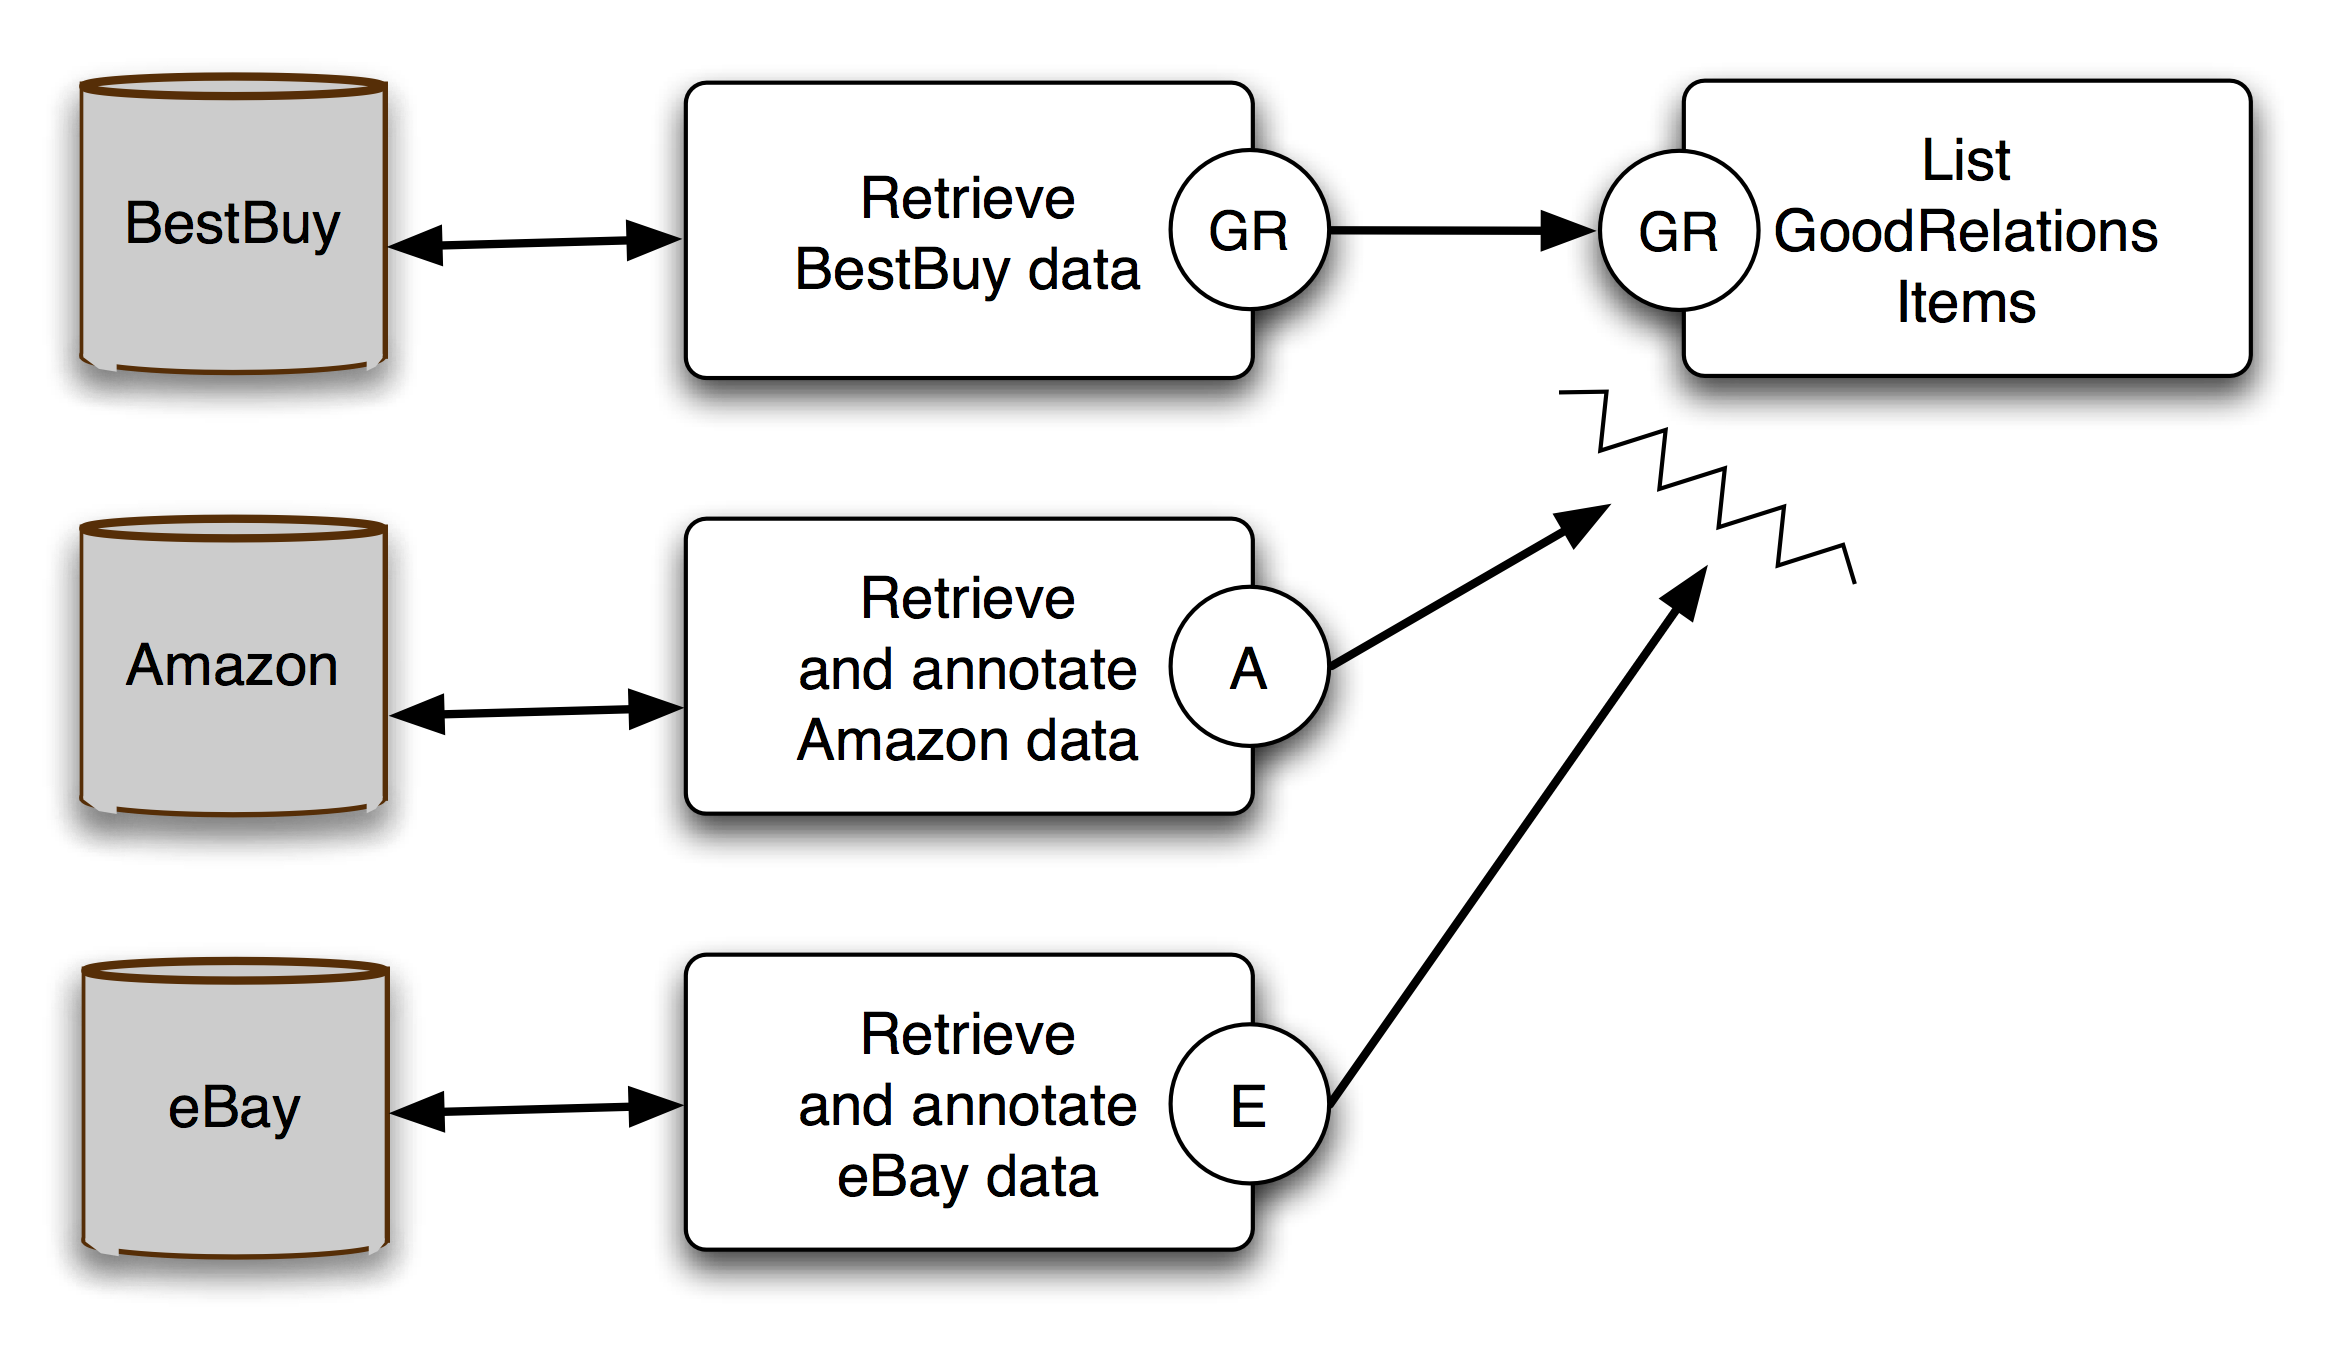
\includegraphics[width=8cm]{images/screens_diagram.png}%[bb=0 0 201 126]
        \caption{Three gadget components retrieving incompatible data}
    \label{fig:screens}
\end{figure}

Figure~\ref{fig:screens} illustrates our scenario. There are three retrieval components that wrap the different e-commerce sites and provide data according to three different ontologies: the GR ontology, the Amazon ontology (A) and the eBay ontology (E). Another component displays GR items for display to the user, but not A or E items. If the gadget designer wants to aggregate data from all three services in the display, there will therefore have to be a mapping present between A and E on the one hand, and GR on the other.

%, say we have a component that accesses the BestBuy service and retrieves RDF data that uses the GoodRelations ontology. In other words, the output of this component is GoodRelations data. Another component takes this data and displays them in a list, i.e. this component only accepts GoodRelations data for display. Since both components use the same ontology, they can be combined. However, now suppose we have two additional components, which access the Amazon and eBay services and retrieve items from there, which are then represented using the Amazon and eBay ontologies, respecitvely. The user wants to list items from all three sources in the same display component. However, since all three ontologies are incompatible, this is not possible out of the box. What is necessary is a mapping between the Amazon and GoodRelations, as well as eBay and GoodRelations ontologies.

%We have thus a case, where we want to aggregate data using three different ontologies, so aligning them to a common ontology is the only possible solution.

\subsection{Ontologies}
\label{ontologies}
Of the three ontologies used in our evaluation, only GoodRelations is a real-world, extensive ontology for e-commerce. The other two, i.e., the Amazon and the eBay ontologies were developed for simulation purposes as simplified versions of what would be used in the real-life scenarios. They were designed to showcase particular features of ontology mapping in our scenario.

\paragraph{GoodRelations:}
This ontology is aimed at annotating so-called ``offerings'' on the Web, which can be products or services. The ontology features support for ranges of units, measurements, currencies,  shipping and payments, common business functions (sell, lease, repair, etc.) and international standards (ISO 4217 or UNSPSC) and codes (e.g., EAN or UPC) in the field.
The main class is \texttt{Offering},
which represents an announcement by a \texttt{BusinessEntity} to provide a \texttt{ProductOrService} with a given \texttt{BusinessFunction}. It may be constrained in terms of eligible business partner, countries, quantities, and other properties. It is also described by a given \texttt{PriceSpecification}. The super-class for all classes describing products or service types is \texttt{ProductOrService}. This top-level concept has sub-classes representing actual product instances, product models and dummy product placeholders. A product is described by its title and description, manufacturer, make and model, etc. 
% While GoodRelations offers terminology to allow a much higher expressivity, we will restrict the discussion to those terms relevant for our scenario.


% \begin{center}
% \lstset{captionpos=b, breaklines=true}
% \lstset{frame=single, basicstyle=\scriptsize}
% \lstset{caption=Basic GoodRelations data in N3 notation, label=listing_gr}
% \lstset{language=XML}
% \begin{lstlisting}
% :Offering_8794691     a gr:Offering;
%   gr:hasPriceSpecification 
%       :UnitPriceSpecification_8794691_1;
%   gr:includesObject :TypeAndQuantityNode_8794691_1;
% 
% :UnitPriceSpecification_8794691_1     a gr:UnitPriceSpecification;
%   gr:hasCurrency "USD"^^xsd:string;
%   gr:hasCurrencyValue "749.99"^^xsd:float;
%   gr:hasUnitOfMeasurement "C62"^^xsd:string;
% 
% :TypeAndQuantityNode_8794691_1     a gr:TypeAndQuantityNode;
%   gr:amountOfThisGood "1.0"^^xsd:float;
%   gr:hasUnitOfMeasurement "C62"^^xsd:string;
%   gr:typeOfGood :ProductOrServicesSomeInstancesPlaceholder_8794691 .
% 
% :ProductOrServicesSomeInstancesPlaceholder_8794691 a gr:ProductOrServicesSomeInstancesPlaceholder;
%   gr:hasEAN_UCC-13 "0013803096095"^^xsd:string;
%   gr:hasMakeAndModel :PoSM_8794691;
%   rdfs:comment "With Auto Optimization and [...]"@en;
% 
% :PoSM_8794691     a gr:ProductOrServiceModel;
%   gr:hasManufacturer <bbuy:Manufacturer_Canon>;
%   rdfs:label "Canon EOS Digital Rebel [...]"@en;
%   rdfs:comment "With Auto Optimization and [...]"@en;
% \end{lstlisting}
% \end{center}


\paragraph{Amazon Ontology:}
We have created a small Amazon ontology based on a subset of the datatypes supported by the web service exposed by Amazon to third-party agents. The ontology describes \texttt{Items} based on the \texttt{ItemAttributes} description given in the Amazon Product Advertising API documentation\footnote{\url{http://docs.amazonwebservices.com/AWSECommerceService/latest/DG/}}.
The ontology features three classes for describing a product. Example instance data is given in List.~\ref{listing_amazon}.
\begin{inparaenum}[(1)]
    \item \texttt{Item} represents an Amazon item, defined by a title, a manufacturer, a product group (DVD, Book, etc.), an international EAN code, an ASIN (unique Amazon id), an author (for books) and a \texttt{ListPrice}. 
    \item \texttt{Company}, described by a  legal name, is used for representing the manufacturer of an \texttt{Item}.
    \item \texttt{ListPrice} has two properties: \texttt{hasCurrencyCode}, representing an ISO 4217 currency code (e.g. GBP or EUR), and \texttt{hasAmount} representing the price in the given currency.
\end{inparaenum}


% \begin{figure}[ht]
\lstset{caption=Simplified Amazon ontology data in N3 notation, label=listing_amazon}
\lstset{language=turtle}
\begin{lstlisting}
:Item_7590645 a amzn:Item;
   amzn:hasASIN "B0012YA85A";
   amzn:hasManufacturer :Manufacturer_Canon;
   amzn:hasModel "XSI Kit";
   amzn:hasPrice :Price_7590645_1;
   amzn:hasProductGroup "Electronics";
   amzn:hasTitle "Canon Digital Rebel XSi [...]" .
:Manufacturer_Canon a amzn:Company;
   amzn:hasLegalName "Canon" .
:Price_7590645_1 a amzn:ListPrice;
   amzn:hasAmount "575.55";
   amzn:hasCurrencyCode "GBP" .
\end{lstlisting}
% \end{figure}

\paragraph{eBay Ontology:}
The eBay ontology was created based on the eBay Shopping API\footnote{\url{http://developer.ebay.com/DevZone/shopping/docs/CallRef/index.html}} and is supposed to annotate data retrieved through the web service described by the API.
% \begin{center}
% \lstset{captionpos=b, breaklines=true}
% \lstset{frame=single, basicstyle=\small}
% \lstset{caption=Simplified eBay ontology data in N3 notation, label=listing_ebay}
% \lstset{language=XML}
% \begin{lstlisting}
% 
% :SimpleItem_1320648     a ebay:SimpleItem;
%   ebay:hasItemID "E012Y090912";
%   ebay:hasBidCount :"4";
%   ebay:hasCountry "UK";
%   ebay:hasCurrentPrice :Price_1320648_1;
%   ebay:hasPrimaryCategoryName "Electronics";
%   ebay:hasTitle "Canon Digital Rebel XSi [...]" .
%   ebay:hasDescription "Camera is practically unused. It's like new."
% 
% :Price_1320648_1     a ebay:CurrentPrice;
%   ebay:hasAmount "575.55";
%   ebay:hasAmountType "GBP" 
% \end{lstlisting}
% \end{center}
The ontology features three basic classes,
%  (see Listing \ref{listing_ebay} for an example of ebay data)
\begin{inparaenum}[(1)]
    \item \texttt{SimpleItem} represents an eBay \texttt{Item}, that is sold by a \texttt{SimpleUser}. It is described by a title, a \texttt{CurrentPrice} (specifying the highest bid, or the selling price of fix-priced items), primary category name, manufacturer, model, EAN code, item ID (a unique eBay ID), bid count, end time of bid, country where the item is located, and a product ID (which supports major international product codes --- this property is from the Finding API).
    \item The \texttt{CurrentPrice} features a \texttt{hasAmountType} property, specifying the currency code, and a \texttt{hasAmount} property, which is the amount of money for a price per unit.
    \item \texttt{SimpleUser} contains information about eBay users. Users are described by a user ID, about me URL and the seller's positive feedback score. This class will not be used for capturing information on goods for our scenario, but is an essential component of the eBay system, which was the reason for its inclusion in the ontology.
\end{inparaenum}

\subsection{Testing and Results}
\label{testing}

We present the approach an ontology engineer has to take to discover and represent ontology mappings, and a means to exploit them after the they have been discovered and appropriately represented.

There is a major paradigm difference between the GoodRelations ontology and the other two ontologies (see Sect.~\ref{sub:manual_mapping} for details). After some initial testing, we concluded that automatic mapping from GR to A/E using the string-based methods employed by the Alignment API tool was not feasible. Therefore, the following sections report on \emph{automatic mapping} for the A--E pair --- which are similar enough to be suitable for level 0 mapping ---, and \emph{manual mapping} for the GR--A/E pairs.

\subsubsection{Automatic Mapping}
\label{subsubsec:automaticmapping}

% \paragraph{The Matcher} % (fold)
% \label{par:the_matcher}

% paragraph the_matcher (end)
For automatic mapping of level 0 mappings, we used a simple string distance-based algorithm provided by Alignment API~\cite{euzenat2004api}, which computes the string distance between the names of the entities to find correspondences between them. Four methods have been used for computing the distance:
\begin{inparaenum}[(1)]
    \item equality, which tests whether the names are identical, 
    \item Levenshtein distance (number of character operations needed), 
    \item SMOA distance (which is a specialised distance for matching ontology identifiers) and
    \item a Wordnet-based~\cite{fellbaum1998wordnet} distance using the JWNL library with Wordnet.
\end{inparaenum}

The alignment description derived from these methods is given based on a simple vocabulary, containing a pair of ontologies and a set of correspondences, which express relations between entities of the two ontologies.
We used the level 0 mapping representation for representing simple mappings, which map discrete entities of the two ontologies. Thus the representation of the correspondences is given with the five elements described (with the \texttt{id} being optional), as shown in List.~\ref{listing_correspondence}. Similar mappings were were also used for more complex, manually-created representations (level 2), as detailed in Sect.~\ref{sub:manual_mapping}.

% \begin{figure}[ht]
% \begin{minipage}{\linewidth}
\lstset{caption=Level 0 mapping element example, label=listing_correspondence}
\lstset{language=turtle}
\begin{lstlisting}
<level_0_mapping> a align:Cell;
  align:entity1 amzn:hasCurrencyCode;
  align:entity2 ebay:hasAmountType;
  align:measure "1.0"^^xsd:float;
  align:relation "=" .
\end{lstlisting}
% \end{minipage}
% \end{figure}

% \subsubsection{Using the Tool.}
% The Alignment API tool can be used through a GUI, as a server or from the
% command-line interface, of which we have chosen the last one.
% The tool reads two RDF/OWL ontologies, computes the alignment between them, 
% performs some thresholding and displays the results. It can render the output
% in a number of formats, including HTML and XSLT.
% 
% An additional feature of the tool is its ability to evaluate results based on
% a reference alignment, and output the evaluation results in a table,
% or plot them as \LaTeX{} graphs.

\paragraph{Testing Procedure}
For the Amazon--eBay pair we set up a reference alignment, against which the results are evaluated.
We then ran the matching process for all for methods:
\begin{inparaenum}[(1)]
    \item equality,
    \item Levenshtein distance with a confidence threshold of \texttt{0.33} (meaning that any correspondence having a smaller confidence measure will be excluded),
    \item SMOA distance with a threshold of \texttt{0.5} and
    \item Wordnet distance using a threshold of \texttt{0.5}\footnote{Thresholds were selected based on suggestions in the Alignment API documentation}.
\end{inparaenum}
To apply the results, we rendered an XSLT template to transform an example dataset.

\paragraph{Results}

The results of automatically aligning the Amazon and eBay ontologies were quite favourable. As shown in Tab.~\ref{table_results}, we captured the four main parameters used in information retrieval, as described in \cite{olson2008advanced}. These four parameters are used for evaluating the performance of the alignment methods: 
\begin{inparaenum}[(1)]
    \item \textit{Precision}, the fraction of results that are correct --- the higher, the better, 
    \item \textit{Recall}, the ratio of the correct results to the total number of correct correspondences --- the higher, the better, 
    \item \emph{Fallout}, the fraction of incorrect results - the lower the better, and 
    \item \emph{F-measure}, which measures the overall effectiveness of the retrieval by a harmonic mean of precision and recall --- the higher, the better.
\end{inparaenum}

\begin{table}
    \centering
    \caption{Alignment results: Precision, Recall, Fallout and F-Measure}
    \label{table_results}

    \begin{tabular}{rrrrr}
        \toprule
        & \textbf{precision} & \textbf{recall} & \textbf{fallout} & \textbf{f-measure}\\
        \midrule
        \textbf{reference} & 1.00 & 1.00 & 0.00 & 1.00\\
        \textbf{equality} & 1.00 & 0.38 & 0.00 & 0.55\\
        \textbf{SMOA} & 0.43 & 0.75 & 0.57 & 0.55\\
        \textbf{Levenshtein} & 0.40 & 0.75 & 0.60 & 0.52\\
        \textbf{JWNL} & 0.67 & 0.75 & 0.33 & 0.71\\
        \bottomrule
    \end{tabular}
\end{table}

The first row (reference) shows the reference alignment, which, naturally, has both perfect precision and recall. We can observe what intuition has predicted, namely that pure string equality on term labels is far too simple and therefore irrelevant. By using string distances and giving certain thresholds (``Levenshtein and SMOA''), we can see that the results are much less precise, but have a better recall, since this allows for entities having similar names to be discovered, at the expense of having quite a few incorrect results; the thresholds allow for low-scored cases to be eliminated, although this results in the exclusion of some correct correspondences. The last row (``JWNL'') contains the results of the Wordnet-enabled method, which shows quite an improvement (precision of 0.67 and a recall of 0.75),
% \footnote{The scores are orientative, giving a general picture of how the process approaches 100\% efficiency}
due to the lexical analysis, which performs a much more relevant comparison of strings, giving a high number of correct results. The precision of the JWNL alignment shows only a tiny drop below the recall value, meaning that the number of incorrect correspondences discovered is small, and the main source of error is from the number of correspondences not discovered.


% \begin{center}
% \begin{figure}
% %% Plot generated by GenPlot of alignapi
% \begin{center}
% \begin{tikzpicture}[cap=round, scale=0.75]
% % Draw grid
% \draw[step=1cm,very thin,color=gray] (-0.2,-0.2) grid (10.0,9.0);
% \draw[|-|] (-0,0) -- (10,0);
% %\draw[dashed,very thin] (0,0) -- (5,8.66) -- (10,0);
% \draw[dashed,very thin] (10,0) arc (0:60:10cm);
% \draw[dashed,very thin] (0,0) arc (180:120:10cm);
% \draw (0,-0.3) node {$precision$};
% \draw (10,-0.3) node {$recall$};
% % Plots
% \draw plot[mark=+,] coordinates {(5.0,8.660254037844386)};
% \draw (5.01,8.370254037844385) node[anchor=south west] {Reference};
% \draw plot[mark=+,] coordinates {(9.296875,3.6834922606644636)};
% \draw (9.306875,3.3934922606644633) node[anchor=south west] {Equal};
% \draw plot[mark=+,] coordinates {(3.1058673469387754,2.9531229168449795)};
% \draw (3.115867346938775,2.6631229168449793) node[anchor=south west] {SMOA0.5};
% \draw plot[mark=+,] coordinates {(2.9875000000000003,2.6598578439458005)};
% \draw (2.9975,2.3698578439458003) node[anchor=south west] {Levenshtein0.33};
% \draw plot[mark=+,] coordinates {(4.409722222222222,4.99987943527481)};
% \draw (4.419722222222222,4.70987943527481) node[anchor=south west] {JWNL};
% 
% \end{tikzpicture}
% \end{center}
% \caption{Comparison of the four methods, against the reference alignment,\newline
% showing the distances from 0 precision and 0 recall}
% \label{fig:figure_alignment}
% \end{figure}
% \end{center}


We can deduce that the results provided are satisfactory, even though the methods used were simple, string-based ones, and the process was completely automated without any user input.
We are therefore confident that through some user assistance or an initial input alignment the tool can achieve 100\% correct results, which is our aim for the tool to be used in practice.


% \paragraph{XSLT:}
% One of the appealing features of the Alignment API is that it can render the results in XSLT, thus specifying a set of rules which make it possible to transform an  XML file from one format to the other. We have generated such an XML transformation description, and with the simple Linux application \texttt{xsltproc} (run from the command line) we have managed to transform data (limited, of course by the incompleteness of the alignment) from the Amazon ontology into data annotated by the eBay vocabulary. 
%Please refer to Appendix A for a listing of an example transformation.

\subsubsection{Manual Mapping} % (fold)
\label{sub:manual_mapping}

The GoodRelations ontology employs a unique paradigm, different from the paradigms of Amazon and eBay. In GR everything is centred around an instance of \texttt{Offering} and a graph of other instances attached to it, whereas for Amazon (and similarly for eBay), the main class is \texttt{Item}, which holds all relevant properties. In principle, \texttt{Item} would correspond to \texttt{ProductOrService} in GoodRelations, but the properties of the \texttt{Item} class are reflected as properties of many different classes in GR. 

Though the infeasibility of automating this alignment became obvious, we have represented the alignment in the mapping language supported by the tool, as a level 2 mapping (described in Sect.~\ref{mediation}).
 % (the mapping has been created between Amazon and GoodRelations, since the eBay and Amazon ontologies are very similar in approach, and mapping eBay to GoodRelations would be an indentical task). 
This mapping description can later be used by the run-time gadget code. List.~\ref{listing_gr_a} shows an example mapping between two properties of the two ontologies, specifying that the relationship is \texttt{Equivalence} with a certainty degree of \texttt{1.0}. This fragment does not show, but assumes the equivalence correspondence between the classes \texttt{Item} and \texttt{Offering}, which is a trivial level 0 mapping. This mapping specifies the relation

\begin{equation*} \label{eq}
\begin{split}
\forall{v,z}; hasEAN(v,z) & \Longrightarrow \exists{x, y}; includesObject(v,x) \wedge \\
&typeOfGood(x,y) \wedge hasEAN\_UCC\_13(y,z),
\end{split}
\end{equation*}

meaning that the \texttt{hasEAN} property of \texttt{v} in the Amazon ontology corresponds to the \texttt{hasEAN\_UCC\_13} property of the \texttt{typeOfGood} of the \texttt{includesObject} of \texttt{v} in GoodRelations. The domains and ranges of the properties are inferred, thus it is deduced, that in \texttt{Amazon v} is of type \texttt{Item} and \texttt{z} is \texttt{int}, and in \texttt{GoodRelations v, x, y} and \texttt{z} are instances of the classes \texttt{Offering}, \texttt{TypeAndQuantityNode}, \texttt{ProductOrService} and \texttt{int}, respectively.

\begin{figure}[ht]
\lstset{caption=Fragment of the Amazon--GoodRelations mapping, label=listing_gr_a}
\lstset{language=turtle}
\begin{lstlisting}
<level_2_mapping> a align:Cell;
   align:entity1 amzn:hasEAN;
   align:entity2 
      [ a align:Property;
        align:first gr:includesObject;
        align:next gr:hasEAN_UCC_13,
           gr:typeOfGood ];
     align:measure "1.0"^^xsd:float;
     align:relation "Equivalence" .

amzn:hasEAN a align:Property .
gr:hasEAN_UCC_13 a align:Property .
gr:includesObject a align:Relation .
gr:typeOfGood a align:Relation .
\end{lstlisting}
\end{figure}

% \begin{center}
% \lstset{caption=Fragment of the Amazon--GoodRelations mapping, label=listing_gr_a}
% \lstset{language=xml}
% \begin{lstlisting}
% <Cell rdf:about="MappingRule_01">
%  <entity1><omwg:Property rdf:about="&amzn;hasEAN"/></entity1>
%  <entity2>
%   <omwg:Property>
%     <first><Relation rdf:about="&gr;includesObject"/></first>
%     <next><Relation rdf:about="&gr;typeOfGood"/></next>
%     <next><Property rdf:about="&gr;hasEAN_UCC_13"/></next>
%   </omwg:Property>
%  </entity2>
%  <measure rdf:datatype="&xsd;float">1.0</measure>
%  <relation>Equivalence</relation>
% </Cell>
% \end{lstlisting}
% \end{center}

Using this representation, complex correspondences can be modelled, using first order logic constructs.

\subsection{Fact Transformation Tool}
\label{sec:fact_tool}

To support the application of previously created mapping rules, we have developed a rule based, interactive \emph{fact transformation tool} (or \emph{fact tool} for short). This tool utilises techniques of our service wrapper tool. One part of the service wrapper tool~\cite{rivera2011connecting} uses a rule-based approach for the transformation of web service responses into FAST facts (i.e., instances of ontology concepts). The application of ontology mediation rules can be modelled in a similar vein. In the fact tool, we therefore use analogous rule-based techniques to create data transformation operators, i.e., operators that mediate between two different conceptualisation.

\begin{figure}
    \centering
    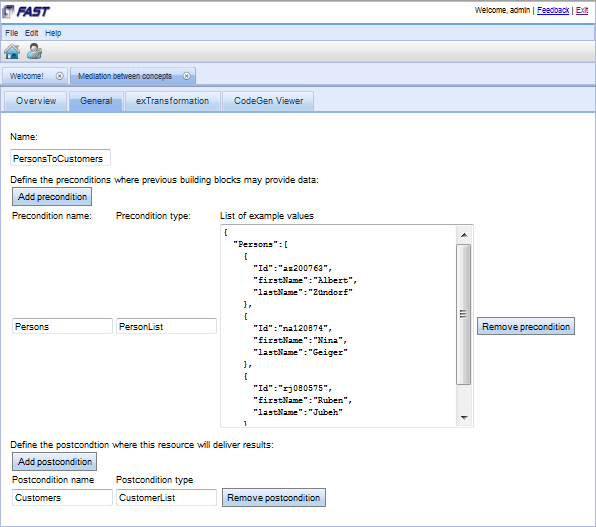
\includegraphics[width=0.8\linewidth]{images/GVSMediationToolPreconditions.png}
    \caption{Definition of operator pre- / postconditions}
    \label{fig:FactsTransformationToolPortDefinitions}
\end{figure}

Figure \ref{fig:FactsTransformationToolPortDefinitions} shows a screen shot of the  fact transformation tool within the GVS environment. The tool has four tabs\footnote{The \texttt{CodeGen Viewer} tab is explained later in Sect.~\ref{sec:runtime}.}, of which the \textit{General} tab (currently shown in the screen shot) is employed to define the pre- and postconditions for the desired data transformation operator in a first general step. 
Using the terminology introduced previously, this allows to define a basic \emph{level 0} mapping between two concepts (\texttt{PersonList} and \texttt{CustomerList} in the example).
The fact tool communicates with the FAST catalogue to select concepts and provide example instances (as JSON data structures) that help the user to perform the correct choice.
% These conditions are typed according to the participating semantic elements to be derived from the FAST catalogue. This typing will provide the structure of the input and output data of the desired data transformation operator.  
After this step, the mapping can be refined to a higher level by defining concrete transformation rules. These can be edited in the \emph{exTransformation} tab as shown in Fig.~\ref{fig:FactsTransformationToolTransformationRules}. On the left of the tab the user is presented with a tree of example data for the input concept, while the right side of the tab shows a similar tree with the derived data for the output concept. This way, the user can continuously observe the effect of changes in the rule they are currently editing. The fact tool constantly executes the transformation rules after any editing, giving direct feedback on their effect and thus enabling the user to validate the achieved transformation. 

\begin{figure}
  \begin{center}
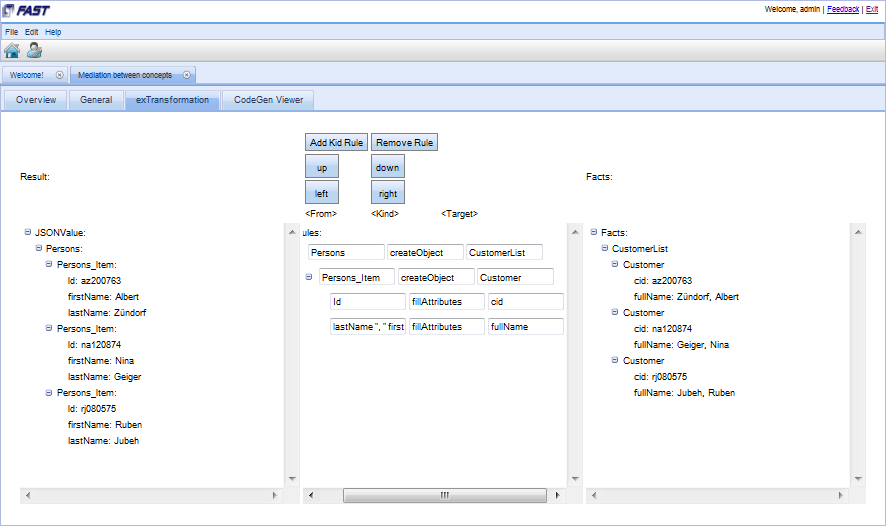
\includegraphics[width=\linewidth]{images/FactsTransformationToolGVSWithTransformationRules.png}
    \caption{Interactive, rule-based transformation of Person facts}
    \label{fig:FactsTransformationToolTransformationRules}
  \end{center}
\end{figure}

Examples for the rules themselves are shown in the rule tree in the middle of Fig.~\ref{fig:FactsTransformationToolTransformationRules}. Starting with a root rule, additional rules can be added as child-rules, while existing rules can be moved around the tree or deleted. Rules can have different types, such as \emph{createObject} or \emph{fillAttributes}. A \textit{createObject} rule can be used to create output fact objects. The \textit{Target} field of such a rule specifies the type of the created objects (i.e., a concept from the FAST catalogue), in our example \textit{List}. The top rule fires for each element of the input data with the type specified in the \textit{From} field of the transformation rule. Thus, in our example, the input data is searched for objects of type \textit{List} firing for the root of our data. The second rule of our example creates \textit{Customer} objects. This rule is a sub-rule of the root rule and thus the created objects are added to the \textit{List} object created by the parent rule. Similarly, the search for triggering objects of type \textit{Person} is restricted to the subtree below the from element that has triggered the parent rule, i.e. to our input \textit{List}. The third rule is used to fill the attribute \textit{fullName} of the \textit{Customer} objects. This rule is an example for a many-to-one transformation. The result is a string concatenation of the \textit{lastName} of the \textit{Person} that has triggered the parent rule plus a text constant plus the \textit{firstName} of the current \textit{Person}. The resulting string is transferred to the \textit{fullName} attribute of the corresponding \textit{Customer}. 

Note that simple one-to-one transformation rules may be derived with the help of the ontology mediation approach described in Sect.~\ref{subsubsec:automaticmapping}. Such simple rules can be added to the transformation tool, automatically. The more complex rules may then be added interactively. During editing, the semantics provided by the FAST catalogue are used to support the user with completion proposals and consistency checking. In addition, the direct execution of the rules on example data helps the user to create appropriate rules and to validate their effects. 

So far our transformation rules are restricted to simple cases. We have focused on simple cases allowing a simple transformation approach that does not require sophisticated skills from our users. 


\subsection{Creating the Operator}
\label{sec:creating_the_operator}

Once the data transformation operator has been defined, it may be added to the FAST catalogue in order to allow its use for the definition of piping configurations of new screens within the FAST GVS tool. For this purpose a simple semantic description is sent to the FAST catalogue defining the semantics of the operator and the semantics of its pre- and postconditions. This is shown in Fig.~\ref{fig:operator_in_screen_builder}, where the newly created data transformator for mediating between Person and Customer concepts (i.e., transforming instances of one concepts into instances of the other) has been saved and is now available in the GVS screen builder interface as an filter operator. 

\begin{figure}[h]
  \begin{center}
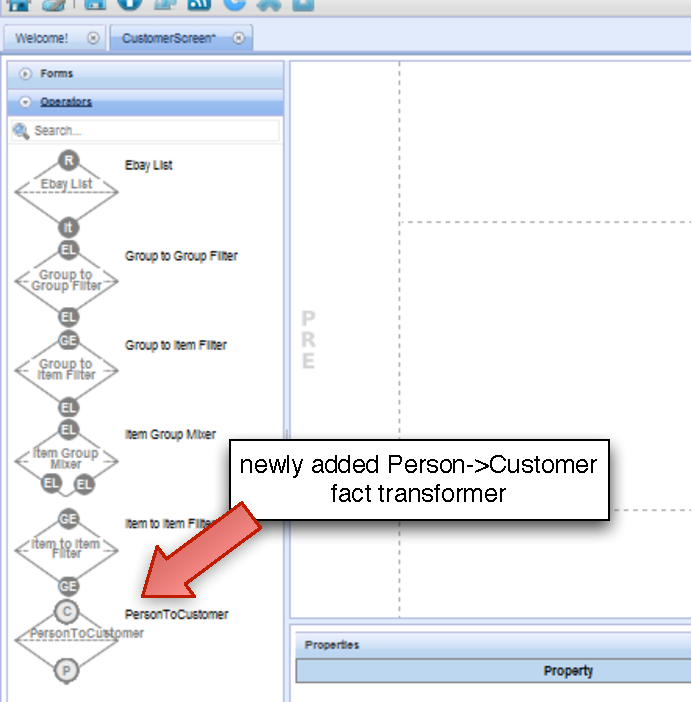
\includegraphics[width=.6\linewidth]{images/operator_closeup}
    \caption{A newly created operator in the GVS screen builder}
    \label{fig:operator_in_screen_builder}
  \end{center}
\end{figure}

The Service Wrapper Tool uses its own repository for trees of transformation rules. First of all this has technical reasons: the development of the transformation tool is based on a reference architecture and libraries for web-based interactive systems provided by Kassel University~\cite{AsDH2009CVSM}. This repository has the special advantage that it provides support for teams of developers, thus the service wrapper tool allows to merge the contributions of multiple developers. 


\section{Gadget Building  and Runtime}

Neither gadget (or screenflow) building or runtime are directly involved with the ontology mapping process. However, the steps performed previously affect these phases of the lifecycle as well, as discussed briefly in the sections below.

\subsection{Gadget Building} % (fold)
\label{sec:gadgetbuilding}

Every time ontology matching is performed and an alignment is created between two underlying resources, the corresponding alignment rules are stored and an operator building block is created in the catalogue, to be available during screen development. 

During the gadget building phase, whenever pre- and post-conditions of screens, resources or operators show a semantic mismatch, the catalogue offers the possible matching operators that would solve the incompatibility problem. This way a matching operator can be placed between two pre- and postconditions that would otherwise be incompatible, making interoperation between the two possible. In seldom cases, the catalogue may fail to retrieve an appropriate mediation operator. In such cases, the possibility of building a new mapping operator with the help of the fact transformation tool is presented, allowing the user to assume the role of ontology engineer in special cases.  

\subsection{Runtime} 
\label{sec:runtime}
For deployment, the gadget's implementation is generated as an executable bundle containing a portion of Javascript code. In addition, a small FAST runtime library (again Javascript) is added to the gadget. This runtime library provides notification mechanisms and manages the fact base of the gadget. For data transformation purposes (i.e., ontology mapping) we generate Javascript code that connects itself to the fact base. Any time a fact is sent to the pre-condition of the operator, it performs the data transformation and sends the result to the post-condition. The code generated from the transformation rules follows a recursive pattern, where each rule is represented as a Javascript function with parameters for the source and target fact subtrees to be transformed. The function body then uses code to search the source tree for sub elements that match the \textit{From} part of the rule and then code for the desired operation is generated. For debugging purposes the user can examine the code generated for an operator in the \textit{CodeGen Viewer} tab of the fact tool. 

Our code generation for service wrappers and transformation operators uses a template-based approach. Thus, the \textit{CodeGen Viewer} tab will also allow to examine the templates used for code generation and to adapt the templates in order to meet changing APIs or to meet new requirements. Thereby, the code generation is not hard wired into our tool but may be adapted by (skilled) end users on the fly. 

\section{Summary}
\label{sec:summary}
With the Semantic Web winning more and more ground both in research and industry, the mismatches between ontologies used by the inter-operating systems present an increasing problem. Ontology matching deals with identifying these mismatches, and overcoming them. 

The initial work on the ontology matching comprised an overview of the area in general, and was reflected in the first iteration of this deliverable (\cite{ambrus2009mediation}, now in App.~\ref{sec:background}). In it, we discussed the theoretical foundations of ontology matching. After presenting the main problem and the types of mismatches between ontologies, we presented --- based on a study of the state-of-the-art in these areas --- the three main approaches to ontology mediation, i.e., \textit{ontology mapping} (representing  correspondences between entities), \textit{ontology alignment} (the process of finding the correspondences between ontologies) and \textit{ontology merging} (the process of creating a new ontology based on the source ontologies that need to be reconciled). 

The second iteration of the document~\cite{ambrus2010mediation} saw a positioning of ontology matching within the FAST project, both in terms of the FAST lifecycle and its associated user roles. It was defined which phases are affected in which way, and which actions by particular user roles are involved. We have shown how matching is done at the different phases of the gadget life cycle and the approach taken at every level. Additionally, we covered different candidates for tools to support automatic matching algorithms and evaluated the most promising ones on the backdrop of an e-commerce scenario. It was found that, while automatic matching is feasible for some, mostly simple cases, the manual definition of mapping rules will still be necessary for many real-life cases. Research into new methods for automatic matching of complex cases was deemed outside the scope of this project. Instead, the focus was on supporting users of the FAST tool to manually define mapping rules in an intuitive fashion. To this end, a first standalone prototype of the \emph{fact transformation tool} was developed and presented briefly.

This final iteration of the deliverable focussed mainly on the improvement of the fact tool and its transformation of a standalone tool into an integral part of the FAST tool chain, thereby supporting users and allowing them to use the same kind of interaction and user interface throughout the platform. The fact tool presented in this deliverable and the service wrapping tool presented in \cite{rivera2011connecting} therefore use a similar graphical approach. Without leaving the FAST platform, users can now assume the role of ontology engineer and define mapping rules of varying complexity, which can then be saved as operator building blocks, to be used in the screen development process. To allow this, the fact tool communicates with the FAST catalogue to guide users in the rule creation process and outputs definitions according to the FAST gadget ontology, as well as code to be used in the deployed gadget.



\section{Summary}
\label{sec:summary}
With the Semantic Web winning more and more ground both in research and industry, the mismatches between ontologies used by the inter-operating systems present an increasing problem. Ontology matching deals with identifying these mismatches, and overcoming them. 

In the first iteration (described in the Appendix) we laid the theoretical foundations of ontology matching. After presenting the main problem, and the types of mismatches between ontologies, we have discussed - based on the most prominent research results in these areas - the three main approaches to ontology mediation, that is \textit{ontology mapping} (representing  correspondences between entities), \textit{ontology alignment} (the process of finding the correspondences between ontologies) and \textit{ontology merging }(the process of creating a new ontology based
on the source ontologies that need to be reconciled). 

In this second iteration (described in the main body of this document) we established the approach to integrate ontology matching into FAST, and we have shown how this matching is done at the different phases of the gadget life cycle and the approach taken at every level. Firstly, we have shown the implementation details as well as test scenarios, we have presented a tool for finding the alignments between ontologies as well as a powerful language to represent them, we have described a tool to compose mapping rules in a consistent manner with other FAST components and the means to save them in the Semantic Catalogue. Secondly, we described the way in which mapping operators are used in the GVS to combine discrepant screens. Lastly, we presented the way the matching operator and mapping rules are deployed and exploited in the JavaScript gadget.

For the last and final iteration of deliverable D2.4 we plan to evaluate real-life scenarios and finalise the implementation of ontology matching for the FAST platform.


%\pagebreak
%\part{D2.4.1: Theoretical Foundations for Ontology Mediation}
%\label{part:d2.4.1}

\clearpage
\phantomsection
\appendix

\section{Ontology Mediation Background}
\label{sec:background}

\subsection{Ontologies}
\label{sec:ontologies}
This section provides a brief introduction to the concept of ontologies.

\subsubsection{Definitions}
As specified in \cite{gruber2008ontology} {\textquotedblleft}an ontology defines a
set of representational primitives with which to model a domain of
knowledge or discourse{\textquotedblright}. These primitives are
typically classes, attributes and relations among classes or class
instances (and others, such as function terms, rules, restrictions,
axioms and events). Their definitions provide information about their
semantics (meaning) and constraints on their logically consistent
usage. 

Ontologies are typically specified in languages that allow to abstract
away from implementation details, and focus on the so-called semantic
level. This way ontologies provide a representation independent from
data models and implementation, thus providing a means to enable
interoperability among disparate systems and specifying interfaces to
independent, knowledge-based systems. In the technology stack of the
Semantic Web, ontologies define a separate layer, and have a set of
languages and tools (both commercial and open-source) to work with
them. 

We would also mention a widely-known and used classical definition of
ontologies, presented in \cite{gruber93towards}: {\textquotedblright}[An
ontology is] an explicit, formal specification of a shared
conceptualisation{\textquotedblright}. \cite{studer1998knowledge_engineering_principles} explains
this definition, by elaborating on the four main terms of the
definition:

\begin{enumerate}
\item it is a conceptualisation, because it models and categorises
relevant concepts from the real world, 
\item it is explicit, because the model explicitly states the types of
the concepts, the relationships between them and the constraints of
their use, 
\item it is formal, because the ontology has to be machine-readable and
consistent, and 
\item it is shared, because an ontology is consensual, i.e. accepted by
a group of people and it is used in a shared environment to allow a
common conceptualisation of data. 
\end{enumerate}

\subsubsection{General Description}
An ontology is used to define the vocabulary that agents use to exchange
queries and assertions. If an agent commits to a common ontology, it
guarantees the consistency (but not completeness) of the queries and
assertions using the vocabulary defined in the ontology \cite{gruber93towards}.
An agent supporting the interface defined in an ontology is not
required to use the terms of the ontology as an internal encoding of
its knowledge. Nonetheless, the definitions and formal constraints of
the ontology do restrict what can be meaningfully stated in the
language defined. 

Two analogies to ontologies are given in \cite{gruber93towards}. Ontologies are
similar to global type declarations in a conventional software library,
and ontological commitments are similar to type restrictions over the
inputs and outputs of program modules. Formal argument restrictions can
be checked mechanically by compilers, to make sure that calling
procedures pass legal data to called procedures. Similarly, sentences
in an exchange between agents can be checked for logical consistency
using the definitions in the ontologies. Just as the formal argument
list hides the internal structure of a procedure from its calling
environment, a common ontology allows one to interact with a
knowledge-based program without committing to or being aware of its
internal encoding of knowledge. 

Ontologies are also like conceptual schemata in database systems. Such a
schema provides a logical description of the data being shared,
allowing applications to interact with it without having any knowledge
of internal data structures. So while a conceptual schema defines
relations and constraints on data, an ontology defines terms with which
to represent knowledge, and constraints on their relationships.
\cite{gruber2008ontology} also points out that the requirement of inputs and
outputs to be logically consistent with the definitions and constraints
of an ontology is analogous to the requirement that the rows of a
database table (or insert statements in SQL) must be consistent with
the integrity constraints imposed on the table, stated separately and
independently of the internal data formats. 

\cite{gruber2008ontology} enumerates the key applications of ontologies, by saying
that they {\textquotedblleft}are part of the W3C standards stack for
the Semantic Web, in which they are used to specify standard conceptual
vocabularies in which to exchange data among systems, provide services
for answering queries, publish reusable knowledge bases, and offer
services to facilitate interoperability across multiple, heterogeneous
systems and databases.{\textquotedblright} The key role of ontologies
in database systems is to provide a data modeling layer above specified
database designs, so that data can be used across independently
developed systems and services. This made it possible to achieve
database interoperability, cross database search and web service
interrogation. 

There are many issues not addressed by common ontologies, related to
knowledge sharing. One important question is how a group of people can
reach a consensus on a common ontology. The discussion of ontology
mediation aims to address this problem by attempting a solution to the
case of several ontologies conceptualising a similar domain of the real
world in different ways.


\subsection{The Mediation Problem} %%%%%%%%%%%%%%%%%%%%%%%%%%%%
\label{sec:mediationproblem}
Ontologies are employed as explicit descriptions of the information
source semantics. According to \cite{wache2001ontology_information_integration}, integrating these
semantics along multiple systems can be done using three main
approaches. (1) The single ontology approach, using a single ontology
as a global shared vocabulary. Unfortunately this can not provide
different views on a domain, and using it for multiple similar
catalogues is unfeasible due to the vast amount of information needed
to be captured, and the susceptibility of the conceptualisation to
change. (2) The multiple ontology approach has each information source
describing its own ontology. This solves problems related to the single
ontology approach, but introduces the problem of differences in
conceptualising the same concepts. Ontology mediation can be used to
map different parts of the ontologies to each other. (3) The hybrid
approach uses multiple ontologies, but uses a global ontology to make
all the ontologies comparable to each other. This is closely related to
ontology merging, where overlapping entities are merged, and the rest
is simply composed into one unified ontology, allowing for the
definition of the concepts of both ontologies. We suggest that the FAST
Gadget Ontology (as defined in D2.1) could act as a global ontology in
the context of FAST, although further research needs to be done in this
direction, since the Gadget Ontology has a slightly different
epistemological commitment. 

In the context of FAST, the problem is that of reconciling the
ontologies in the back-end with the ontologies in the front-end, to
allow for interoperability between the two layers. 

In the following we present a motivating scenario for ontology mediation
in Section \ref{subsec:mediationproblem_motivatingexample}, and a formal description of the alignment problem and
process, respectively, in Section \ref{subsec:mediationproblem_problemstatement}. After that we show some examples
of ontology mediation in Section \ref{subsec:mediationproblem_examples}.

\subsubsection{Motivating Example}
\label{subsec:mediationproblem_motivatingexample}
This section presents a brief example, illustrating a problem that
presents the need for ontology mediation. 

%\begin{verbatim}
\lstset{frame=single, basicstyle=\ttfamily, caption=Ontology \texttt{O1}.}
\lstset{emph={vsmlVariant, namespace, ontology, concept, ofType, instance, nonFunctionalProperties, endNonFunctionalProperties, memberOf, hasValue}}
\lstset{emphstyle=\textbf\textit\underbar}
\begin{lstlisting}
vsmlVariant -"http://www.smo.org/wsml/wsml-syntax/wsml-flight"

namespace { -"http://see.deri.org/adrian/thesis/ontologies/O1#" ,
       wsml - "http://www.wsmo.org/wsml/wsml-syntax#" ,
         dc - "http://purl.org/dc/elements/1.1/" }

ontology - "http://see.deri.org/thesis/ontologies/O1"
    nonFunctionalProperties
    dc#description hasValue "A simple ontology modeling
                             the concept of a person"
    endNonFunctionalProperties

concept person
    name ofType _string
    age ofType _integer
    hasGender ofType gender
    hasChild ofType person
    marriedTo ofType person

concept gender
    value ofType _string

instance male memberOf gender
    value hasValue "male"
instance female memberOf gender
    value hasValue "female"
\end{lstlisting}

Consider the two ontologies \texttt{O1} and
\texttt{O2} \cite{mocan2008mediation} presented in Listing 1 and
Listing 2 respectively, in the Human Readable Syntax of the Web Service
Modeling Language (WSML) \cite{debruin2005wsml}. Elements from
ontology \texttt{O1} need to be mapped to the elements
described in Ontology \texttt{O2}. 

Ontology \texttt{O1} describes the concept
\texttt{person} as one having five attributes, each of
them having a type that is either a concept or a value from a given
data type. The concept gender has two instances defined, that have
attributes pointing to the corresponding values. 

\lstset{frame=single, caption=Ontology \texttt{O2}.}
%\lstset{emph={vsmlVariant, namespace, ontology, concept, ofType, instance, nonFunctionalProperties, endNonFunctionalProperties, memberOf, hasValue}}
%\lstset{emphstyle=\textbf}
\begin{lstlisting}
vsmlVariant -"http://www.smo.org/wsml/wsml-syntax/wsml-flight"

namespace { -"http://see.deri.org/adrian/thesis/ontologies/O2#" ,
       wsml - "http://www.wsmo.org/wsml/wsml-syntax#" ,
         dc - "http://purl.org/dc/elements/1.1/" }

ontology - "http://see.deri.org/thesis/ontologies/O2"
    nonFunctionalProperties
    dc#description hasValue "A simple ontology modeling
                             the concept of a human"
    endNonFunctionalProperties

concept human
    name ofType _string
    age ofType _integer
    noOfChildren ofType _integer

concept man subConceptOf human

concept woman subConceptOf human

concept marriage
    hasParticipant ofType human
    date ofType _date
\end{lstlisting}

%\newline
Ontology \texttt{O2} describes the concept
\texttt{human} as one having three attributes. The
concepts \texttt{man} and \texttt{woman} are
subclasses of the concept \texttt{human}. 

Additionally a fourth concept called \texttt{marriage} is
defined having two attributes. (For simplicity we do not deal with the
exceptions of polygamy and same-sex marriage). 

Suppose that a service (or agent) using ontology O1 needs to interact
with a service accepting and providing data that is semantically
defined in ontology O2. 

The first step is to identify candidates to be mapped or to have
taxonomic relationships under an integrated schema \cite{shvaiko2005schema_based}. It is obvious that \texttt{person} and
\texttt{human} are candidates to be mapped, as well as the
class \texttt{man} with the class
\texttt{person} having the attribute
\texttt{gender} equal to
{\textquotedblleft}\texttt{male}{\textquotedblright} and
the class \texttt{woman} with the class
\texttt{person} having the attribute
\texttt{gender} equal to
{\textquotedblleft}\texttt{female}{\textquotedblright}. 

After having identified these correspondences, the next step is to
generate query expressions and assertions that automatically translate
data instances of one of these ontologies into the other one, or that
automatically handle their semantic relations under an integrated
ontology. 

\subsubsection{Problem Statement}
\label{subsec:mediationproblem_problemstatement}
Given two ontologies \texttt{o} and
\texttt{o{\textquotesingle}} that need to be mapped to
each other, according to \cite{shvaiko2005schema_based} we can define a
mapping element as a 5-tuple \texttt{{\textless}id, e,
e{\textquotesingle}, n, R{\textgreater}}, where 

\begin{itemize}
\item \texttt{id} is a unique identifier, identifying the
mapping element, 
\item \texttt{e} and
\texttt{e{\textquotesingle}} entities (classes,
attributes, relations) of the first and second ontology, respectively, 
\item \texttt{n} is a confidence measure in some
mathematical structure holding the correspondence value between e and
e{\textquotesingle}, 
\item \texttt{R} is the correspondence relation holding
between e and e{\textquotesingle} (e.g.,
\texttt{equivalence (=); more general($\sqsupseteq$); disjointness($\perp$); overlapping($\sqcap$)}.
\end{itemize}

\begin{figure}
    \centering
        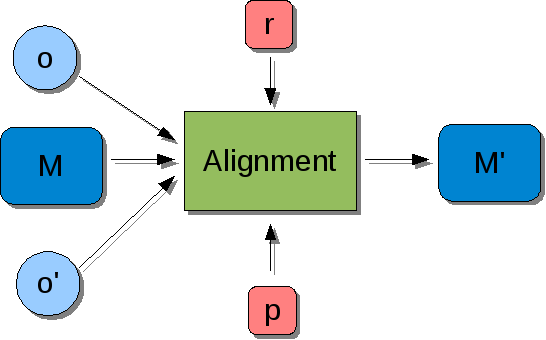
\includegraphics[width=72mm, height=45mm]{images/Alignment_process.png}%[bb=0 0 201 126]
        \caption{The alignment process}
    \label{fig:Alignment}
\end{figure}

A mapping is a set of the above defined mapping elements. The alignment
operation determines the mapping
(M\texttt{{\textquotesingle}}) for the pair of ontologies
(\texttt{o} and
\texttt{o{\textquotesingle}}). There are some parameters
than can extend the definition of the alignment process, namely: 

\begin{enumerate}
\item an input mapping, \texttt{M}, which is to be used and
completed by the process, 
\item the mapping parameters, \texttt{p} (such as weights
and thresholds), that configure the alignment process, 
\item other external resources used by the alignment,
\texttt{r} (such as dictionaries, thesauri, etc.); See Figure \ref{fig:Alignment}. 
\end{enumerate}
For example, suppose that based on some algorithm (using linguistic and
structural analysis) the confidence measure for the equivalence
relation between the classes \texttt{person} in
\texttt{O1} and \texttt{human} in
\texttt{O2} is 0.62. Suppose that a mapping parameter
specifies a threshold of 0.55 for this algorithm, that is all pairs of
entities with a confidence measure higher that 0.55 will be considered
correct mapping elements. Thus our algorithms would return the
following mapping element: \texttt{{\textless} id11,
person, human, 0.62, = {\textgreater}.}Now, another algorithm
determines the two concepts to mean exactly the same thing, thus it
either does not compute a confidence measure (returning
\texttt{n/a}), or it returns the upper limit of the
confidence measure interval (e.g. 1). Thus the mapping element would
be: \texttt{{\textless} id11, person, human, n/a, =
{\textgreater}.} 

It should be noted, that the entities mapped between two ontologies can
be constructed using patterns, i.e. more than just mapping concepts to
concepts, and so on. For example, we can map a concept to a concept
having a certain attribute, like in the case of the concept
\texttt{person} having the attribute
\texttt{hasGender} equal to \texttt{female}
from \texttt{O1} being mapped to the concept
\texttt{woman} from \texttt{O2}. 

\subsubsection{Mediation Examples}
\label{subsec:mediationproblem_examples}
We present two further examples to better illustrate the use of ontology
mediation. 

The first example is taken from \cite{giunchiglia2008evaluation}. Based on the
idea that we view ontologies as graph-like structures, we exemplify
ontology matching with the help of fragments of two tree-like
structures, such as Google and Looksmart. Notice that in the general
case the relation holding between nodes is not specialisation, but
classification (parent-child relation). 

\begin{figure}[h]
    \centering
        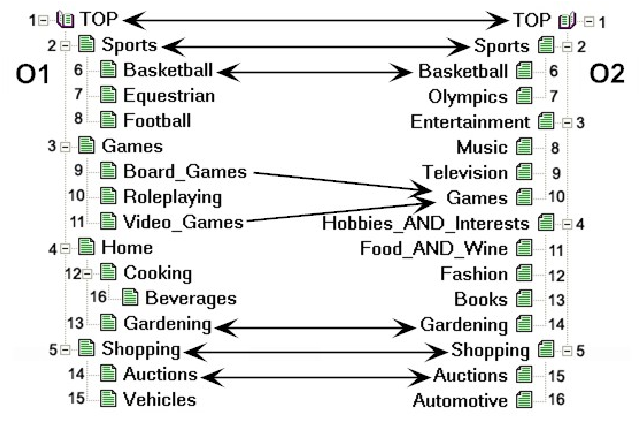
\includegraphics[width=101mm, height=67mm]{images/F2GoogleLooksmart.png}%[bb=0 0 254 167]
        \caption{Fragments of Google and Looksmart directories and some
correspondences. Double arrowheads denote equivalence, while single
arrowheads stand for the more general relation. Image taken from
\cite{giunchiglia2008evaluation}.}
    \label{fig:GoogleLooksmart}
\end{figure}

Suppose we want to merge the merge the two structures. Such situations
can arise, for example when an e-commerce company acquires another one.
One probable mapping is given in Figure \ref{fig:GoogleLooksmart}. We have found, for example,
that \texttt{O1:Basketball} is equivalent to
\texttt{O2:Basketball}, and that
\texttt{O2:Games} is more general than
\texttt{O1:Board\_Games.} 

The second example given in \cite{madhavan2001schema_matching} illustrates the
need to use several techniques in matching two ontologies. Figure \ref{fig:POSchemas}
shows two purchase order schemas that need to be matched. 

\begin{figure}[h]
    \centering
        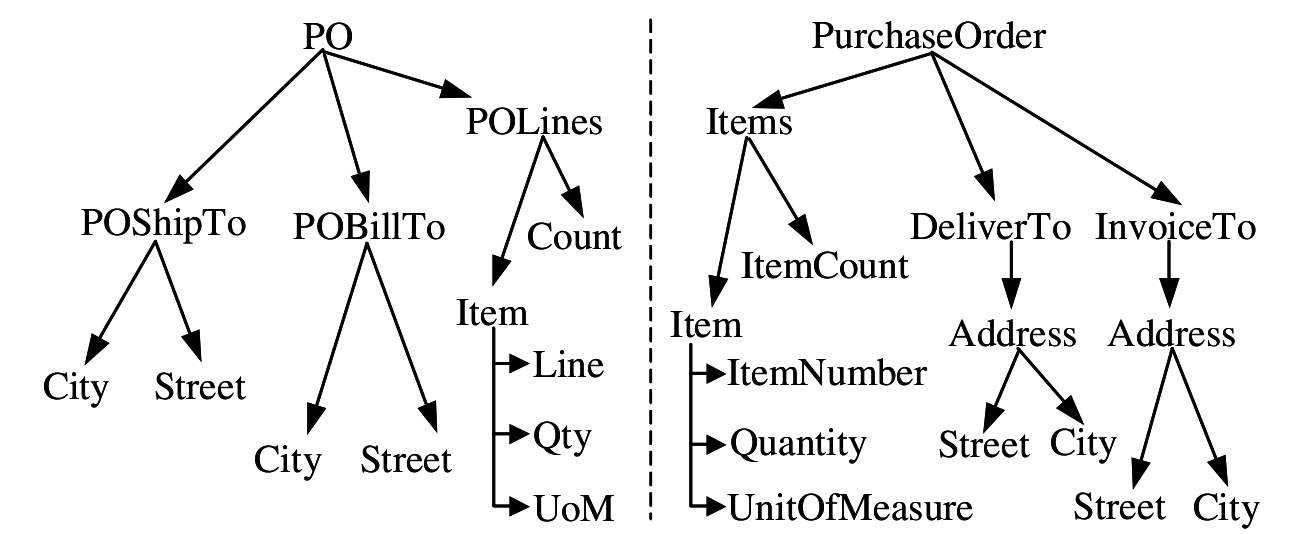
\includegraphics [width=101mm, height=42mm]{images/F1POSchemas.png}%[bb=0 0 257 105]
        \caption{Matching purchase order schemas. Image taken from \cite{madhavan2001schema_matching}.}
    \label{fig:POSchemas}
\end{figure}

As stated above in Section 3.2 we look for similarity coefficients
between the two schemas and deduce a mapping from those coefficients.
Suppose, as a first phase we use linguistic matching, using thesauri to
help match names, acronyms, synonyms, etc. resulting in a set of
candidate pairs (such as \texttt{PO} and
\texttt{PurchaseOrder}, or \texttt{Bill} and
\texttt{Invoice}) and language similarity coefficients
(\texttt{lsim}). In the second phase we would perform a
structural matching of the two schemas. For example,
\texttt{Line} would be mapped to
\texttt{ItemNumber}, because their parents and their other
two children match, \texttt{City} under
\texttt{POBillTo} will be mapped to
\texttt{City} under \texttt{InvoiceTo},
because bill is a synonym to invoice. This process results in
structural similarity coefficients (\texttt{ssim}). By
using a weighted similarity, we can compute the final mappings (e.g. by
using the formula \texttt{wsim=ws*wsim+(1-ws)*lsim}, where
\texttt{ws} is the interval [0,1]). 


\subsection{Ontology Mismatches}
\label{sec:ontologymismatches}
Ontology mismatches are the main obstacles in the combined use of
independently developed ontologies. We will now give an overview of the
main type of ontology mismatches as presented in \cite{klein2001combiningOntologies}, which
is the main source of input to this state-of-the-art report. We will
classify ontology mismatches into given types and will find their
relationships. 

Firstly, two levels of mismatches can be distinguished. The first level
is the \textit{language} or meta-model level. These are differences in
the primitives that make up the language used to specify the ontology.
They produce mismatches in the mechanics to define classes, relations,
attributes and so on. The second level is the \textit{ontology} or
model level. This is were the actual ontology is located. These are
differences in the way the domain is modeled. 

In this section we discuss the overlap and mismatches between concepts,
relations, attributes and instances. We will detail the two levels of
mismatches and the different types that occur at each level. 

\subsubsection{Language Level Mismatches}
\label{subsec:ontologymismatches_languagelevel}
We define four types of mismatches, although they often coincide. These
occur when ontologies written in different languages are combined. We
note that these type of mismatches will be less relevant for FAST
because we assume that standards for ontology languages are now so well
established that in practice we will not very often find ontologies
written in different languages anymore, but we discuss them briefly to
give a better overview of the meditation problem. 

\paragraph{Syntax}
Different languages obviously use different syntax. Therefore the same
concept can (and will be) often modeled in a completely different way.
For example, the concept of chairs would be defined in RDF Schema as
\texttt{{\textless}rdfs:Class
ID={\textquotedblright}Chair{\textquotedblright}{\textgreater}}, while
in LOOM it would be \texttt{(defconcept Chair)}. 

This is the simplest possible mismatch, although it often comes coupled
with other mismatches as well. The simplest form is when a language has
several syntactical forms. 

The solution is to simply to have a rewrite mechanism that returns the
corresponding translated form. 

\paragraph{Logical representation}
A slightly more complicated mismatch is when a logical notion can not be
represented in a given language. For example, in certain languages it
is possible to assert that two classes are disjoint, say using
\texttt{(disjoint A B),} whereas in other languages it is
necessary to express this using simpler statements, such as the
negation of set-inclusion statements, like \texttt{A
subclass-of (NOT B), B subclass-of (NOT A).} 

The actual problem is not the question if something can be expressed,
but finding the language constructs to express a logical notion (not a
concept). 

Solving this mismatch is relatively-easy: it consists in finding
translation rules to transform one representation into another. 

\paragraph{Semantics of primitives}
This difference is a more subtle one, and occurs at the meta-model of
the language. It sometimes occurs that the semantics of an identical
name differs from language to language. For example, the expression
\texttt{A equalsTo B} can have many different
interpretations. 

Even when two ontologies use the same syntax, the semantics may differ.
For example, the OIL RDF syntax interprets several
\texttt{{\textless}rdfs:domain{\textgreater}} statements
as the intersection of the arguments, whereas RDF Schema interprets
them as the union of the arguments. 

\paragraph{Language expressiveness}
This mismatch, at the meta-model level of the languages, is the one
having the greatest impact on the attempt to combine and reconcile
ontologies. 

The difference implies that some languages can express notions that
others can not. For example, some languages have no constructs to
express negation, whereas other do. Other typical examples are support
for sets, lists, etc. 

These type of mismatches have the greatest impact, and are sometimes
mentioned as the {\textquotedblleft}fundamental
differences{\textquotedblright} between knowledge models. 

\subsubsection{Ontology Level Mismatches}
\label{subsec:ontologymismatches_ontologylevel}
Mismatches at the model level happen both in the case of having the two
ontologies written in the same language and syntax and in the case of
different languages. We can distinguish between several types of
ontology level mismatches. 

A conceptualisation mismatch is a difference in how the domain is
modelled (conceptualised), therefore we will have different concepts and
different relations between them. Explication mismatches are
differences in the way the concepts are specified. These occur as
mismatches in definitions, or terms, or the combination of the two.
Terminological mismatches are naming differences or conflicts. Finally,
encoding mismatches are differences in the way values are specified,
for example currencies for prices. 

These kinds of mismatches are likely to occur in the context of FAST and
are therefore important factors in the implementation of ontology
mediation in FAST. 

\paragraph{Conceptualisation Mismatches}
These are differences in the conceptualisation of the domain, that is
not only the specification differs in the two ontologies, but the model
as well. 

Sometimes these mismatches can not be reconciled automatically, and need
a domain expert. In this case, a good solution would be to use both
ontologies together. In that case, the overlapping part needs to be
aligned, and the rest can be merged. 

\paragraph{Scope.}

Two classes that seemingly represent the same concept, but do not have
the same instances, although some of these are identical. For example
the concept of {\textquotedblleft}employee{\textquotedblright} can be
perceived and specified in different ways by different organisations. 

\paragraph{Model coverage and granularity.}
This mismatch is related to the part of the domain that is covered by
the ontologies, and the level of detail respectively. For example, an
ontology could model cars, but no trucks, whereas another would have a
few categories for trucks, and another third ontology could make very
detailed distinction between all the types of trucks and their
properties. 

\paragraph{Explication Mismatches}
The first two types of explication mismatches (\textit{paradigm} and
\textit{concept description}) result from the \textbf{style of
modelling.} The next two types (\textit{synonym terms} and
\textit{homonym terms}) can be classified as \textbf{terminological
mismatches}. Finally, there is one trivial difference, cause by
\textit{encoding} mismatches. 

\paragraph{Paradigm.}
Different paradigms can be used to represent different concepts, or
different top-level ontologies can be used, which all result in this
kind of mismatch. For example, one could model time based on interval
logic, while another could use discrete time points. 

\paragraph{Concept Description.}
These types of mismatches are called modeling conventions. Several
choices can be made in different modeling questions. One choice, the
categorisation of concepts can be done based on an attribute, or using
subclasses. For example, as presented in Section 3.1, the concepts
{\textquotedblleft}man{\textquotedblright} and
{\textquotedblleft}woman{\textquotedblright} can be modeled in several
ways. They could be instances of the concept, and differ only in an
attribute (e.g. \texttt{gender}), or they can be separate
subclasses of a top-level class representing
{\textquotedblleft}humans{\textquotedblright} in general. 

Another choice is the way in which a hierarchy is built - distinction
between features can be made higher or lower in the hierarchy. For
example, consider the place where the difference between scientific and
non-scientific publications is made: a dissertation can be modeled as
\texttt{dissertation }\texttt{{\textless}
book {\textless} scientific publication {\textless} publication}, or as
\texttt{dissertation {\textless} scientific book
{\textless} book {\textless} publication}, or as a subclass of both
\texttt{scientific publication} and
\texttt{book}. 

\paragraph{Synonym Terms.}
Concepts are represented by different names. For example, the term
{\textquotedblleft}car{\textquotedblright} from an ontology can be
represented as {\textquotedblleft}automobile{\textquotedblright} in
another. 

Although the solution looks simple in using thesauri, in reality much
human effort is needed to solve these problems, and care must be taken
not to overlap with scope mismatches (see above). 

\paragraph{Homonym Terms.}
The meaning of a term is different in another context. For example, the
term {\textquotedblleft}conductor{\textquotedblright} has one meaning
in a musical context, and a different meaning in an electric
engineering domain. 

These differences are much harder to solve than synonyms, and always
need human contribution. 

\paragraph{Encoding.}
The values of attributes in ontologies are encoded in different formats.
For example, date can be encoded in a
\texttt{{\textquotedblleft}yyyy-mm-dd{\textquotedblright}}
form, or a
\texttt{{\textquotedblleft}dd/mm/yyyy{\textquotedblright}},
distance might be specified in miles or kilometers, money amount can be
given in different currencies, and so on. 

These kind of mismatches can very easily be solved, by using a wrapper,
or a single transformation step. 


\subsection{Ontology Mediation Approaches}
\label{sec:mediationapproaches}
In this section we give an overview of some of the major approaches to
ontology mediation, following the structure of Section 2: Approaches in
Ontology Mediation of \cite{debruin2005wsml}. Firstly, in Section
\ref{subsec:mediationapproaches_ontologymapping} we present some representative approaches to the specification of
mappings. Then in Section \ref{subsec:mediationapproaches_ontologyalignment} we overview some of the main approaches
and algorithms to overcome mismatches and find mappings between
ontologies, that is we discuss the topic of ontology alignment. Finally
in Section \ref{subsec:mediationapproaches_ontologymerging} we discuss the process of merging several ontologies.
Further research is needed to decide on the type of ontology mediation
to be used in the context of FAST, the algorithms and approaches
applied, and whether to use alignment or merging. 

\subsubsection{Ontology Mapping}
\label{subsec:mediationapproaches_ontologymapping}
An ontology mapping is a declarative specification of the semantic
overlap between two ontologies \cite{debruin2005wsml}. It is the
result of the ontology alignment process (see Figure 3.). This mapping
is usually expressed as a set of axioms in a certain mapping language. 

There are three main phases of the mapping process: (1) discovering the
mapping, (2) representing the mapping and (3)
using/exploiting/executing the mapping. This section is focused on (2),
that is we survey a number of approaches in representing ontology
mappings. 

A common tendency in ontology mapping is to create an ontology of
mappings, which represents the vocabulary for the representation of
mappings. 

\paragraph{MAFRA.}
MAFRA \cite{maedche2002mafra}, or MApping FRAmework for distributed
ontologies supports the interactive, incremental and dynamic process of
ontology mapping, which transforms instances of a source ontology into
instances of a target ontology. 

\subparagraph{Framework Components.}
The framework consists of five main phases (called horizontal
dimensions) and for components that run along the entire process,
called vertical components. Within the horizontal dimension, the
authors identified five modules: 

\begin{itemize}
\item \textit{Lift \& Normalisation}. Both ontologies must be normalised
to the uniform representation of RDFS. As a result both ontologies are
represented in RDF Schema with their instances in RDF. Thus syntactical
end lexical differences are eliminated and semantic differences become
more apparent. 
\item \textit{Similarity.} This module establishes similarities between
entities using different approaches (\textit{lexical similarity},
\textit{property similarity} based on properties of concepts,
\textit{bottom-up similarity} propagating the similarity from lower
parts of the taxonomy to the upper part and \textit{top-down
similarity} that assumes special relevance when top level concepts have
a higher or lower similarity). 
\item \textit{Semantic Bridging}. Based on the similarities computed in
the previous phase, correspondences are identified between entities,
using so-called semantic bridges, which define the actual mapping. 
\item \textit{Execution}. Transforms instances between the two
ontologies using the semantic bridges. 
\item \textit{Post-processing.} Revisiting the mapping for improvements.

\end{itemize}
The vertical dimension contains modules like evolution (synchronising
changes between in the ontologies and the bridges), the GUI (extensive
graphical support must be given for human assistance of the process),
etc. 

\subparagraph{Semantic Bridges.}
Semantic bridges are captured in the Semantic Bridging Ontology (SBO).
Five dimensions have been identified for the semantic bridges, as
presented in the following: 

\begin{itemize}
\item \textit{Entity dimension.} Semantic bridges may relate to the
following entities: (i) concepts modeling object classes from the real
world, (ii) relations modeling relationships of objects, (iii)
attributes modeling simple properties and (iv) extensional patterns
modeling the content of instances. 
\item \textit{Cardinality dimension.} Defines the number of entities on
both sides of the semantic bridge (mostly 1:1, 1:n and m:1; m:n is
rarely encountered, and can be usually decomposed onto m:1:n). 
\item \textit{Structural dimension.} Reflects on how elementary bridges
may be combined into more complex bridges. Relations that hold among
bridges are \textit{specialisation} (reuse a bridge and provide
additional information), \textit{abstraction} (should only be used as a
super-class), \textit{composition} (a bridge is composed of other
bridges) and \textit{alternatives} (mutually exclusive bridges). 
\item \textit{Constraint dimension.} Permits to control the execution of
the semantic bridge. Constraints must hold on the source ontology in
order for the transformation procedures to be applied. 
\item \textit{Transformation dimension.} Reflects on how instances of
the source ontology are transformed during the mapping process. 
\end{itemize}
The Semantic Bridging Ontology (SBO) contains a specification of all
semantic bridges, organised in a taxonomy. To actually relate the
source and the target ontology the mapping process creates an instance
of the SBO containing semantic bridge instances along with all the
necessary information to transform instances of entities from the
source to the target ontology. 

The five semantic bridge dimensions are employed as follows: 

\begin{itemize}
\item There are three basic entity types: \textit{Concepts},
\textit{Relations} and \textit{Attributes}. 
\item The class \textit{SemanticBridge} is the most generic bridge type.
It defines the relations to the source and target entities. It is
specialised according to entity type and cardinality of the relation. 
\item The class \textit{Service} can reference resources that are
responsible to connect to, or to describe transformations. 
\item \textit{Rule} is the general class for constraints and
transformation-relevant information. 
\item The class \textit{Transformation} uses the \textit{inService}
relation to link to the transformation procedure. 
\item The class \textit{Condition} represents the conditions that need
to be satisfied in order to execute the semantic bridge. 
\item The Composition primitive can be accomplished using the
\textit{hasBridge} relation of \textit{SemanticBridge}, without any
cardinality or type constraint. 
\item The Alternative primitive is supported by the
\textit{SemanticBridgeAlt} class. It groups several mutually exclusive
bridges, of which the first consistent bridge (with satisfied
conditions) is executed. 
\end{itemize}
For an extensive and relevant example please refer to Section 3.3. of
\cite{maedche2002mafra}.

\paragraph{RDFT.}
RDFT \cite{omelayenko2002rdft} is a small language (meta-ontology) defined for
mapping XML DTDs to/and RDF Schemas specially targeted for business
integration tasks. It is built on top of RDF Schema and it is used to
map RDF Schemas and concepts like events, messages, vocabularies to
XML-specific parts of the conceptual models that occur in the
integration tasks. 

The model is derived from WSDL \cite{christensen2001wsdl} and provides
an RDF Schema for RDF annotations of WSDL documents, and is extended
with the temporal ontology PSL. The business integration task in this
context is seen as a service integration task, where each enterprise is
represented as a Web service specified in WSDL. WSDL annotations made
according to the defined meta-ontology allow performing inference over
WSDL descriptions to validate the links established between the
enterprises. 

\subparagraph{PSL.}
To be able reason about the inputs and outputs of the companies being
integrated, the authors developed a conceptual model of WSDL, which is
directly derived from the WSDL specification. WSDL defines the
following basic elements of services, on top of which PSL is built: 

\begin{itemize}
\item \texttt{Types} that provide links to the XML Schemas
of the messages exchanged; 
\item abstract definitions of \texttt{Messages} in
accordance with \texttt{Types}; 
\item \texttt{Port} \texttt{Types} that
specify input and output messages; 
\item \texttt{Bindings} that specify concrete protocols and
formats for messages according to \texttt{Types}. 
\end{itemize}
These elements can describe services but do not represent any temporal
knowledge about the messages requiring integration. The Process
Specification Language or PSL temporal ontology includes classes to
capture temporal knowledge: 

\begin{itemize}
\item \texttt{activity} , which is performed during a
certain time interval; 
\item \texttt{activity} \texttt{occurrence} ,
contains the snapshot of an activity at a moment in time; 
\item \texttt{timepoint} , marks the time interval of the
activity; 
\item \texttt{objects} , things that do not possess
temporal properties, but may participate in certain activities at given
time points. 
\end{itemize}
\subparagraph{RDFT.}
The basic RDFT class is \texttt{Bridge }that connects two
concepts. It describes common properties of bridges, which enables one
to specify correspondences between an entity and a set of entities.
allowing for one-to-many and many-to-one connections. 

The bridges contain the \texttt{Relation} property,
pointing to one of the subclasses of
\texttt{BridgeRelation}: 

\begin{itemize}
\item \texttt{EquivalenceRelation}, stating that the source
element is equivalent with the target set of elements, or the source
set of elements is equivalent to the target element respectively,
depending on the relation cardinality; 
\item \texttt{VersionRelation}, specifying that the target
set of elements forms a later version of the source set of elements.
Unlike equivalence bridges, assumes that both concepts belong to the
same domain. 
\end{itemize}
Several types of bridges are defined in RDFT: 

\begin{itemize}
\item \texttt{Event2Event} bridges link different events,
specify temporal event generation conditions, and link the events to
the messages transmitted with them. They connect instances of the
meta-class \texttt{mediator:Event}. 
\item two kinds of \texttt{RDFBridges}:
\texttt{Class2Class} and
\texttt{Property2Property} bridges between RDF Schema
classes and properties. They contain \texttt{rdfs:Class
}and \texttt{rdfs:Property} instances, respectively. 
\item four kinds of \texttt{XMLBridges}:
\texttt{Tag2Class}, \texttt{Tag2Property},
\texttt{Class2Tag}, \texttt{Class2Property},
which link XML DTD tags and RDF Schema classes and properties. 
\end{itemize}
The bridges are grouped into \texttt{Maps}, which are
collections of bridges serving a single purpose. The maps are
identified by their names and form minimal reusable modules of RDFT
bridges. Each map can include other maps and serves as a container for
\texttt{Bridges}. Described in this manner, as a set of
bridges, mappings are said to be \textit{declarative}, while
\textit{procedural} mappings can be defined as Xpath \cite{clark1999xpath} expressions, transforming instance data. 

Connecting two services with RDFT consists of connecting their events
(instantiating \texttt{EventMap}) consisting of
\texttt{Event2Event} bridges. Each of the bridges points
to a \texttt{DocumentMap} aligning the documents attached
to the bridges and, in turn, consisting of
\texttt{RDFBridges}, \texttt{XMLBridges} and
\texttt{VocabularyMaps}. 

\paragraph{C-OWL.}
C-OWL \cite{bouquet2004cowl} gives another perspective on ontology
alignment, extending the widely-known OWL \cite{dean2004owl}
language. 

\subparagraph{The Vision.}
In their vision, similar to the one discussed at the beginning of
Section 3, two types of domain conceptualisations exist: 

\begin{itemize}
\item \textit{ontologies}, that encode a view common to a set of
different parties. They make it easy to exchange information, although
they have the requirement of common consensus and the problem of hard
maintenance. 
\item \textit{contexts}, that encode the view of a party, and are local
conceptualisations, that are not shared. These are easy to maintain,
and no consensus is required, but need explicit mapping among the
contexts of different parties to be able to exchange information. 
\end{itemize}
In this vision, an ontology is contextualised, i.e. it is a
\textit{contextual} \textit{ontology}, when its contents are kept local
(therefore not shared) and can be mapped to the contents of other
ontologies via explicit mappings, allowing for a controlled form of
global visibility. This is opposed to the OWL importing mechanism,
where a set of local models is globalised in a unique shared model, by
importing complete models and using the imported elements by direct
reference. 

\subparagraph{Context OWL.}
Context OWL or C-OWL is a language that extends OWL both syntactically
and semantically to support the concept of contextual ontologies. 

Therefore a contextual ontology defined in C-OWL is a pair consisting
of: 

\begin{enumerate}
\item an OWL ontology, and 
\item mapping between contexts, namely a set of bridge rules with the
same target ontology. 
\end{enumerate}
A C-OWL mapping therefore is a 4-tuple having the following form: 

\begin{enumerate}
\item a mapping identifier (URI), 
\item a source context containing an OWL ontology (URI of the ontology),

\item a target context containing an OWL ontology (URI of the ontology),

\item a set of bridge rules form the local language of the source
ontology to the local language of the target ontology. Each mapping is
composed of three elements: 

\begin{enumerate}
\item a source element (concept, role or individual) of the source
ontology; 
\item a target element, which must be of the same type as the source
element; 
\item the type of mapping (subsuming($\sqsupseteq$), equivalence(=), disjointness($\perp$) and
overlapping($\sqcap$)). 
\end{enumerate}
\end{enumerate}
Thus C-OWL has the complete representational power of OWL, augmented
with appropriate local model semantics for mapping between contexts
(local ontologies). A nice property of C-OWL is that the two components
(the OWL ontology and the mapping) are orthogonal, thus one can use the
ontology or the contextual component in an independent manner. 

The local model semantics defined in C-OWL, as opposed to OWL, considers
that each context has a local set of models and a local domain of
interpretation. Thus, it is possible to have contradicting axioms or
unsatisfiable ontologies in the local models, without having the entire
context space unsatisfiable. 

\subsubsection{Ontology Alignment}
\label{subsec:mediationapproaches_ontologyalignment}
\subsubsection{The Match Operator}
Ontology alignment is the process of discovering similarities between
two source ontologies \cite{debruin2005wsml}. This process can be
described as the application of the so-called \textit{Match} operator
described in \cite{rahm01survey}. The result of the matching
process is a specification of the similarities between the two
ontologies. The input of the Match operator consists mainly of two
ontologies and some other inputs (initial mapping that will be
extended, mapping parameters that configure the process and external
resources used by the matching process; see Section 3.2). 

The generic implementation of the Match operator should contain a
uniform internal representation of the schemas to be matched, in order
to significantly reduce complexity. This, of course, requires a
semantics-preserving schema importer and exporter, respectively. 

In general it is not possible to fully automate the matching between two
ontologies, primarily because they often have semantics that affects
the matching criteria, but is not formally expressed or often even
documented. Therefore the implementation of Match should determine
match candidates, which the user can accept, reject, or change.
Furthermore the user should be able to specify matches for elements for
which the system was unable to find satisfactory match candidates. 

\paragraph{The Alignment Process}
The alignment process proposed in \cite{debruin2005wsml} relieves the user of
some of the burdens in creating the mappings. The input of the process
consists of two ontologies which are to be aligned. The output is a set
of mappings. 

The steps of the alignment are as follows: 

\begin{enumerate}
\item \textit{Feature engineering}. Selects only parts of an ontology
definition in order to describe a specific entity. A feature may be as
simple as a label or it may include super- and sub-concepts, relations
or extensional descriptions.\newline
For example, suppose a fragment of an ontology describes the instance
\texttt{Daimler}. In this case we should consider the
generic ontology feature called type which has the values
\texttt{luxury} and \texttt{automobile},
respectively. 
\item \textit{Selection of Next Search Steps}. This step chooses the
next set of candidate pairs. It may choose to compute a restricted
subset of candidate concept pairs of the two ontologies and ignore the
others. 
\item \textit{Similarity Assessment.} Determines the similarity degree
of candidate pairs. Heuristics are used, that is similarity functions
such as on strings, object sets, related concepts, and so on.\newline
For example, one similarity function can check whether the parents of
the compared two concepts are identical. 
\item \textit{Similarity Aggregation}. For a candidate pair we can (and
often do) use several similarity functions. The results of these
functions need to be aggregated to compute the final similarity measure
between the two entities. This can be done by either a simple
averaging, or a complex aggregation function using weighting schemes. 
\item \textit{Interpretation}. This step uses the aggregated similarity
values to align entities. It can use thresholds for similarity, perform
relaxation labelling, or combine structural and similarity
criteria.\newline
For example, suppose \texttt{simil(o1:Person,
o2:Human)=0.62 ${\geq}$ 0.5}, thus it is added to the result as a
mapping element. 
\item \textit{Iteration}. Several algorithms perform more than one
iteration in order to bootstrap the amount of structural knowledge.
Iteration may stop when no new alignments are proposed, or when a given
number of mappings have been discovered. Note that certain steps can be
omitted in later iterations, since we can use previously computed
values (such as selecting features, computing a given similarity,
etc.). 
\end{enumerate}
The output of the process is a set of correspondences between entities
of the two ontologies. We cannot expect all correspondences to be
discovered, therefore the results of the alignment process can be
considered as the input to a manual refinement process. 

\paragraph{Classification of Approaches}
An implementation of Match may use multiple matching algorithms or
\textit{matchers. }This allows us to select matchers according to the
application domain or schema types. 

Given that we want two use multiple matchers we distinguish two
subproblems. First, there is the need to realise individual matchers,
each of which uses a single matching criterion to find mappings.
Second, we want to combine different individual matchers, either by
using multiple matching criteria within an integrated \textit{hybrid}
\textit{matcher}, or by combining multiple match results provided by
different match algorithms within a \textit{composite}
\textit{matcher}. 

For individual matchers, we consider the following mostly-orthogonal
classification criteria (of which the first one is the most important
distinctive criterion): 

\begin{itemize}
\item \textit{instance-based/schema-based} matching: A schema-based
matcher uses different  \linebreak approaches to determine correspondence between
ontologies based on concepts and relations \cite{debruin2005wsml}. 
An instance-based matcher takes instances
(i.e. instance data) belonging to the different concepts in the
ontologies and uses these to discover similarities between the concept.

\item \textit{element-level/structure-level} matching: an element-level
matcher takes individual schema elements, properties of the particular
concept or relation, and uses these to find similarities, whereas a
structure level matcher compares the combination of elements, the
structure (e.g. the concept hierarchy) of the ontologies to find
similarities. 
\item \textit{language/constraint}: a matcher can use a linguistic
approach (e.g. based on names and textual description of schema
elements) or a constraint-based approach (e.g. based on keys and
relationships). 
\item \textit{matching cardinality:} an overall matching result can
relate one or more elements of an ontology to one or more elements of
the other, giving four cases: 1:1, 1:n, m:1 and n:m. In addition each
mapping element can may interrelate one ore more elements of the given
ontologies. Furthermore, there may be different cardinalities at the
instance level. 
\item \textit{auxiliary information}: most matchers rely on external
information besides the two given ontologies, such as global schemas,
dictionaries, previous matching decisions and user input. 
\item \textit{accepted input:} this dimension concerns the type of input
on which the algorithms operate, classified depending on the
data/conceptual models they accept. 
\item \textit{produced output}: this pertains to the way the mapping is
described, whether it is a one-to-one correspondence or a more general
one, whether it is a graded answer (98\% or 4/5), or an all-or-nothing
approach, whether the result focuses only on equivalence between
entities, or can it give a more expressive result, and so on. 
\end{itemize}

\paragraph{Schema-based matching.}
A schema-based matcher \cite{rahm01survey} takes different aspects
of the concepts and relations in ontologies and uses some similarity
measure to determine correspondence. The available information includes
the usual properties of ontology elements, such as name, description,
data types, relationship types (part-of, is-a, etc.), constraints and
ontology structures. In the following we discuss some of the main
aspects of schema-based matching. 

\begin{itemize}
\item \textit{Granularity of match}. We distinguish two main
alternatives, element-level and structure-level matching. For each
element of the fist ontology, an \textit{element-level matcher}
determines the matching element of the second ontology at the same
granularity level (usually at the atomic level). For instance, in two
ontology fragments describing addresses we could find that
\texttt{{\textquotedblleft}Address.ZIP}{\textquotedblright}
from one ontology matches
{\textquotedblleft}\texttt{CustomerAddress.PostalCode{\textquotedblright}}
from the other one. \textit{Structure level matching}on the other hand
refers to matching combinations of elements that appear together in a
structure. This can be a complete, or a partial match. Known
equivalence patterns can be kept in a library. For example (this
conforms to a common equivalence pattern), one ontology could have a
class \texttt{ParttimeEmployee}, which is the subclass of
\texttt{Employee}, while another could have a class
\texttt{Employee} having the attribute
\texttt{IsParttime}. A structure-level matcher should
identify these as being identical, when the
\texttt{IsParttime} property equals to true. 
\end{itemize}
\begin{itemize}
\item \textit{Match cardinality}. An element can participate in zero,
one or many mapping elements of a match result. Moreover, within a
mapping element, one or more elements from one ontology can match one
or more elements from the other one. Thus we have the usual
relationship cardinalities of 1:1, n:1, 1:m and n:m between matching
elements, both with respect to different mapping elements
(\textit{global cardinality}) and with respect to an individual mapping
element (\textit{local cardinality}).\newline
Most existing matchers map each element of one schema to one element of
the other schema. This results in local 1:1 mappings and global 1:1 or
1:n mappings. 
\end{itemize}
\begin{itemize}
\item \textit{Linguistic approaches}. Linguistic matchers use name and
text (i.e. words or sentences) to find semantically similar elements.
\textit{Name matching} matches elements with identical or similar names
(using synonyms, common substrings, user-provided name matching, etc.).
\textit{Description matching} uses natural language comments of
ontology elements. For example we can have
{\textquotedblleft}\texttt{empn //employee
name}{\textquotedblright} in an ontology matching
{\textquotedblleft}\texttt{name //name of
employee}{\textquotedblright} in the other. This can be done by simple
keyword extraction, or complex natural language processing. 
\end{itemize}
\begin{itemize}
\item \textit{Constraint-based approaches.} These approaches use the
fact that ontologies often contain constraints on data types and
ranges, relationships, optionality, uniqueness, cardinalities, etc.
This information can be used to determine similarities between ontology
elements. For example, in a candidate pair having the fields
\texttt{Born} and \texttt{BirthDate}
respectively, both having the type \texttt{Date}, a
constraint-based matcher could find these to be similar. 
\end{itemize}
\begin{itemize}
\item \textit{Reusing schema and mapping information}. In addition to
already mentioned auxiliary information, matchers could well reuse
common ontology components and previously determined mappings. Some
mappings occur very often in the same domains, and reusing these
increases effectiveness. For example, in e-commerce domains
substructures often repeat with different message formats (like
address, name, etc.), so we could keep a library of previously found
results on these, so when we find two elements labelled
\texttt{ProductOrder} and \texttt{Product} in
an ontology \texttt{O1}, and \texttt{Porder}
and \texttt{Article} in an ontology
\texttt{O2}, the matcher would already know that these
match (\texttt{ProductOrder} matches
\texttt{POrder} and \texttt{Product} matches
\texttt{Article}). 
\end{itemize}

\paragraph{Instance-based matching.}
An instance-based matcher \cite{rahm01survey} takes instances
(i.e. instance data) belonging to the different concepts in the
ontologies and uses these to discover similarities between the
concepts. It can be useful when the data is semistructured or
particularly useful to uncover incorrect interpretations of schema
information. 

The approaches we discuss for instance-level matching primarily work in
finding element-level matches, because of the complexity of comparing
large numbers of combinations of instances. 

Most of the approaches of schema-level matchers can be applied here, but
some are especially applicable: 

\begin{itemize}
\item For text elements, a linguistic approach based on information
retrieval techniques is the preferred approach. For example, if we have
a field called \texttt{Dept} in an ontology, and two
fields \texttt{DeptName} and \texttt{EmpName}
in another, instance information may help to deduce that
\texttt{DeptName} is the primary match candidate for
\texttt{Dept}. 
\item For more structured data, such as numerical or string elements, we
can apply a constraint-based characterisation, such as numerical value
ranges or character patterns. For instance, this may help recognising
phone numbers, postal codes, birth dates, ISBNs, money-related entries
(e.g. based on currency symbols), etc. 
\end{itemize}
The results of instance-based matchers can be used to enhance
schema-level matchers as a first approach. For instance, a
constraint-based schema-level matcher can more accurately determine
data types and ranges for an element using the results of
instance-based matching. A second approach is to perform instance-level
matching on its own. Matching elements from the first ontology to the
second one, and then vice-versa, we can obtain schema-level matches.
Instance-level matching can also be performed by using auxiliary
information. This is especially helpful for matching text elements by
providing match candidates for individual keywords. For example, a
previous analysis may have revealed that the keyword
\texttt{{\textquotedblleft}HP{\textquotedblright}}
frequently occurs for ontology elements
\texttt{{\textquotedblleft}CompanyName{\textquotedblright}},
\texttt{{\textquotedblleft}Manufacturer{\textquotedblright}},
etc. For a new match task, if an \texttt{O2} ontology
element \texttt{X} frequently contains the term
\texttt{{\textquotedblleft}HP{\textquotedblright}}, this
can be used to generate
\texttt{{\textquotedblleft}CompanyName{\textquotedblright}}
in \texttt{O1} as a match candidate for
\texttt{X}, even if
\texttt{{\textquotedblleft}HP{\textquotedblright}} does
not often occur in instances of \texttt{O1}. 

\paragraph{Overview of Approaches}
In this section we give a brief overview of some of the main approaches
to ontology alignment. 

\paragraph{Anchor-PROMPT.}
Anchor-PROMPT \cite{noy2000anchor_prompt} uses a set of heuristics to analyse
non-local context, as opposed to algorithms like PROMPT \cite{noy2000prompt} 
(See Section \ref{subsubsec:mediationapproaches_ontologymerging_PROMPT}) and Chimaera, that only analyse local context.
It doesn{\textquotesingle}t provide a complete solution, but augments
existing methods. 

The algorithms takes as input two pairs of related terms (anchors) from
the source ontologies. These anchors are either given by the user, or
generated automatically with string-based techniques or another matcher
using linguistic similarity. 

From this set of anchors, the algorithm produces a set of new pairs of
semantically close terms. To do that, Anchor-PROMPT traverses the paths
between the anchors in the corresponding ontologies. A path follows the
links between the classes, defined by the hierarchical relations or by
slots and their domain and range. Anchor-PROMPT then compares these
terms along the paths to find similar terms. Terms with a high
similarity score are presented to the user to improve the set of
possible suggestions, for example, a merging process in PROMPT. 

For example, suppose we have ontology \texttt{O1} having
the classes \texttt{A-C-E-H} in a hierarchical chain, and
\texttt{O2} having the classes
\texttt{B-D-F-G} in its hierarchy. Then, suppose we
identify the anchors as \texttt{A-B} and
\texttt{G-H}. We then traverse each path in parallel,
incrementing the similarity score of the classes we encounter at each
step. We repeat the the process for all existing paths between the
anchor points, cumulatively aggregating the similarity score. 

The central observation behind Anchor-PROMPT is that if two pairs of
terms are similar and there are paths connecting the terms, the
elements along those paths are often similar as well. 

\paragraph{GLUE.}
GLUE \cite{doan2004ontology_matching} applies machine learning techniques to
semi-automatically create semantic mappings between heterogeneous
ontologies based on instance data. It regards ontologies as being
taxonomies of concepts, and focuses on finding 1-to-1 correspondences
between the concepts of the ontologies: for each concept node in one
taxonomy, find the most similar concept node from the other taxonomy. 

Instead of committing to a certain similarity definition, it computes
the \textit{joint probability distribution} of the concepts involved,
and lets the application use the joint distribution to compute any
suitable similarity measure. Specifically, for any two concepts
\texttt{A} and \texttt{B} the joint
probability distribution consists of \texttt{P(A,B),
P(A,{\textlnot}B), P({\textlnot}A,{\textlnot}B)}, and
\texttt{P({\textlnot}A,B),} where a term such as
\texttt{P(A,{\textlnot}B)}, is the probability that an
instance in the domain belongs to concept \texttt{A}, but
not to concept \texttt{B}. 

Computing this joint distribution is based on the sets of instances that
overlap between the two concepts. A term such as
\texttt{P(A,B)} can be approximated as the fraction of
instances that belong to both A and B, that is we need to decide for
each instance whether it belongs to \texttt{A${\Pi}$B}.
GLUE addresses this by using the instances of \texttt{A}
to learn a classifier for \texttt{A}. Then classifies
instances of \texttt{B} according to that classifier, and
vice-versa.

\paragraph{Semantic Matching.}
Semantic Matching \cite{giunchiglia2004semantic_matching} is an implementation of
the Match operator, that takes two graph-like structures (like database
schemas or ontologies) and produces a mapping between elements of the
two graphs that correspond semantically to each other. The authors
argue that most previous approaches used syntax driven techniques, like
matching labels(substrings, abbreviations, similar soundex) or
syntactical structure and calculating a similarity measure, all being
different variations of syntactic matching, that searches for semantic
correspondences based on syntactic features. 

Semantic matching has the following main features: 

\begin{itemize}
\item searching is done by mapping meanings (concepts), not labels. It
is not sufficient to consider the meaning of labels in the nodes, but
also the positions the nodes have in the graph. 
\item semantic similarity relations are used between elements (concepts)
instead of syntactical similarity relations. In particular, those
relations are considered, which relate the extensions of the concepts
under consideration. 
\end{itemize}
The semantics of a node is given by the concept attached to that node
(the concept denoted by the label of the node), by the position of the
given node in the graph, and the semantics of all the nodes which are
higher in the hierarchy. 

The possible returned relations between elements are equality,
overlapping, mismatch, and more general/specific. 

\paragraph{QOM.}
QOM \cite{ehrig2004qom} was designed to create an efficient matching
tool for on-the-fly creation of mappings between ontologies. 

Given that the a major ingredient of run-time complexity is the number
of mapping pairs which have to be compared to actually find the best
mappings, QOM uses heuristics to lower the number of candidate
mappings, thus not comparing all entities of the first ontology to all
entities of the second ontology. It uses the ontological structures to
classify candidate mappings into promising and less promising pairs,
using a dynamic programming approach to refine the set of candidate
mappings in each iteration. 

The similarity measure is computed using a wide range of similarity
functions, such as string similarity. Several of such similarity
measures are computed, which are all input to the similarity
aggregation function, which computes the actual similarity measure. QOM
then applies a sigmoid function, which emphasises high individual
similarities and deemphasises low individual similarities. The actual
correspondences are then extracted using a threshold to the aggregated
similarity measure. 

The output of one iteration of QOM can be used as part of the input of a
subsequent iteration in order to refine the result. After a number of
iterations the actual mapping between the ontologies is obtained. 
\paragraph{Alignment Examples}
This section provides a few examples of the matching
process{\textquotesingle} results.
\begin{center}
\tablecaption{Constraint-based matching example. {\newline}Taken from \cite{rahm01survey}.}
\label{tab:ConstraintMatching}
\tablehead{}
%begin{supertabular}{|r@{\hspace{6.5mm}}|r@{\hspace{5.5mm}}|r|r|}
\begin{supertabular}{|m{0.4\textwidth}|m{0.4\textwidth}|}
\hline
S1 elements &
S2 elements\\\hline
Employee

\ \ \ \ EmpNo -- int, primary key

\ \ \ \ EmpName -- varchar (50)

\ \ \ \ DeptNo -- int, references 

\ \ \ \ Salary -- dec (15,2)

Department

\ \ \ \ Birthdate -- date

\ \ \ \ DeptNo -- int, primary key

\ \ \ \ DeptName -- varchar (40) &
Personnel

\ \ \ \ Pno - int, unique

\ \ \ \ Pname -- string

\ \ \ \ Dept -- string

\ \ \ \ Born -- date\\\hline
\end{supertabular}
\end{center}
The two schemas (corresponding to ontologies) shown in Table \ref{tab:ConstraintMatching} present
an example of constraint-based schema-level matching \cite{rahm01survey}. Type and key information suggest that
\texttt{Born} matches \texttt{Birthdate} and
\texttt{Pno} matches either \texttt{EmpNo} or
\texttt{DeptNo} (this could be refined using
instance-based matching, which could reveal that
\texttt{Pno} matches \texttt{EmpNo}). By
using a matcher that detects more than just atomic-level similarities,
we match \texttt{S2.Personnel }to
\texttt{S1.Employee} joined with
\texttt{S1.Department.} This can be detected automatically
by observing that elements of \texttt{S2.Personnel} match
elements of \texttt{S1.Employee} and
\texttt{S1.Department} and that
\texttt{S1.Employee} and
\texttt{S1.Departmen}t are connected by the foreign key
\texttt{DepNo}. This allows us to determine the correct
SQL-like n:m mapping:
\begin{verbatim}
    S2.Personnel (Pno, Pname, Dept, born) ~
    SELECT S1.Employee.EmpNo,
           S1.Employee.EmpName,
           S1.Department.DeptName,
           S1.Employee.Birthdate
    FROM S1.Employee, S1.Department
    WHERE (S1.Employee.DeptNo = S1.Department.DeptNo)
\end{verbatim}


Table \ref{tab:CardinMatching} \cite{rahm01survey} illustrates match cardinalities for
two given schemas S1 and S2. When matching multiple elements, we can
see that expressions are used to combine them.

\begin{center}
\tablecaption{Matching cardinalities example. {\newline}Taken from \cite{rahm01survey}.}
\label{tab:CardinMatching}
\tablehead{}
\begin{supertabular}{|p{0.20\textwidth}|p{0.20\textwidth}|p{0.20\textwidth}|p{0.20\textwidth}|}
\hline
\textbf{Local match cardinalities} & \textbf{S1 element(s)} & \textbf{S2 element(s)} & \textbf{Matching expression} \\\hline 
1:1, element level & Price & Amount & Amount = Price \\\hline 
n:1, element-level & Price, Tax & Cost & Cost ={\newline}Price*(1+Tax/100) \\\hline 
1:n, element-level & Name & FirstName,\newline
LastName & FirstName,{\newline}LastName =\newline
Extract (Name, \ldots) \\\hline 
n:1 structure-level
(n:m element-level) & B.Title,\newline
B.PuNo,\newline
P.PuNo,\newline
P.Name & A.Book,
A.Publisher & A.Book, A.Publisher =\newline
SELECT B.Title, P.Name\newline
FROM B, P\newline
WHERE B.PuNo=P.PuNo
\\\hline
\end{supertabular}
\end{center}
In the first row, the
match is 1:1, which is the most simple to determine. Row 2 shows how
\texttt{Cost} can be matched to a formula based on
\texttt{Price} and \texttt{Tax}. Row 3
explains how \texttt{FirstName} and
\texttt{LastName} are extracted from
\texttt{Name}. Row 4 uses a SQL expression combining
attributes from two tables. It corresponds to an n:m relationship at
the attribute level (four \texttt{S1} attributes
correspond to two \texttt{S2} attributes) and to an n:1
relationship at the structure level (two tables from
\texttt{S1} match one table from
\texttt{S2}).


\begin{center}
\tablecaption{Class by attribute mapping pattern and example. {\newline}Taken from \cite{debruin2005wsml}.}
\label{tab:MappingPattern}
\tablehead{}
\begin{supertabular}{|m{0.8\linewidth}|}
\hline
\textbf{Name}: Class by Attribute Mapping \\\hline
\textbf{Problem}: The extension of a class in one ontology
corresponds to the extension of a class in another ontology, provided
that all individuals in the extension have a particular attribute
value. \\\hline
\textbf{Solution:} 

\textit{Solution description}: A mapping is established
between a class/attribute/attribute value combination in one ontology
and a class in another ontology. 

\textit{Mapping syntax:} 

\texttt{mapping ::= classMapping(direction A
B attributeValueCondition(P o))} \\\hline
\textbf{Example:} 

\texttt{classMapping(Human Female
attributeValueCondition(hasGender
}{\textquotedblleft}female{\textquotedblright})) \\\hline
\end{supertabular}
\end{center}

The example in Table \ref{tab:MappingPattern} \cite{debruin2005wsml} shows a mapping element from the
motivating example from Section \ref{subsec:mediationproblem_motivatingexample}. Assume we have two ontologies
\texttt{O1} and \texttt{O2} which both
describe humans and their gender. Ontology \texttt{O1}
describes the concept \texttt{Person} with an attribute
\texttt{hasGender}, which has the two possible values
{\textquotedblleft}\texttt{male}{\textquotedblright} and
{\textquotedblleft}\texttt{female}{\textquotedblright}.
Ontology \texttt{O2} describes the concept
\texttt{Human}, and its subclasses
\texttt{Man} and \texttt{Woman} to
distinguish the gender.

Notice that this is a typical case of a
conceptual mismatch, namely a mismatch in the style of modeling. The
solution illustrates an elementary mapping pattern. The pattern is
described in terms of its name,the problem addressed, the solution of
the problem, both in natural-language description and in terms of the
actual mapping language, and an example, namely a mapping between a
class \texttt{Human} from ontology
\texttt{O1} to the class \texttt{Woman} from
ontology \texttt{O2}, but only for humans having the
gender
{\textquotedblleft}\texttt{female}{\textquotedblright}.

\subsubsection{Ontology Merging}
\label{subsec:mediationapproaches_ontologymerging}
Ontology merging is the creation of a new ontology from one or more
source ontologies. The new ontology will unify and in general replace
the original source ontologies. 

We distinguish between two main approaches to ontology merging. In the
first approach the input of the process is a collection of ontologies
and the output is a new, merged ontology which captures the original
ontologies. A prominent example of this is PROMPT \cite{noy2000prompt}. 
In the second approach the ontologies are not replaced, but
rather a {\textquotesingle}view{\textquotesingle}, called
\textit{bridge ontology} is created which imports the original
ontologies and specifies the correspondences using bridge axioms.
OntoMerge \cite{dou2002ontology_translation} is an example of this approach, creating a
bridge ontology that imports the original ontologies and relates the
overlapping concepts in these ontologies using bridge axioms. We
describe PROMPT and OntoMerge in more detail below. 

\paragraph{PROMPT}
\label{subsubsec:mediationapproaches_ontologymerging_PROMPT}
PROMPT \cite{noy2000prompt} is an algorithm and interactive tool for
ontology merging and alignment. It was one of the first ontology
merging tools, comparing every pair in the two ontologies and looking
for syntactic similarity between labels. It has been implemented as a
Proteg\'e-2000 extension. 

The algorithm of PROMPT defines a number of steps for the interactive
merging process: 

\begin{enumerate}
\item An initial list of merging candidates is created, based on class
name similarities. The list is presented to the user as potential
merging operations. Then the following cycle happens: 
\item The user chooses the next operation: selects an option suggested
by the algorithm, or edits the ontology to specify the desired
operation directly. 
\item The third step is composed of the following three sub-steps: 

\begin{enumerate}
\item The system performs the requested action and automatically
executes additional changes derived from the operation. 
\item A new list of suggested operations is presented to the user, based
on the structure of the ontology around the arguments of the last
operation. 
\item The system determines the conflicts introduced by the last
operation and finds possible solutions to them. 
\end{enumerate}
\end{enumerate}
PROMPT defines the following set of ontology-merging operations: merge
classes, merge slots, merge bindings between a slot and a class,
perform a deep copy of the class (copy all parents up to the root),
perform a shallow copy of the class. 

The conflicts that may appear as a result of these operations are: name
conflicts, dangling references, redundancy in the class hierarchy,
slot-value restrictions that violate class inheritance. 

The result of the algorithm is a new ontology which replaces the
original ones. 

\paragraph{OntoMerge}
OntoMerge \cite{dou2002ontology_translation} is an online ontology translation system,
which translates a dataset to a new dataset which captures the same
information in a different ontology. 

The approach divides the process into two main parts, namely separating
the syntactic translation from the semantic translation: 

\begin{enumerate}
\item Converting the datasets into a uniform internal representation (a
language called Web-PDDL) in order to clear away syntactic differences.

\item Perform the semantic translation from the internal representation
of a dataset in the source ontology to the internal representation of
the a dataset in the target ontology. 
\end{enumerate}
The result of the process is not an ontology replacing the original ones
as in PROMPT, but a bridge ontology that imports the source ontologies
and contains a set of Bridging Axioms, which are translation rules used
to connect the overlapping parts of the source ontologies. The two
source ontologies, together with the set of bridging axioms, are then
treated as a single theory by a theorem prover (optimised for
operations like dataset translation, ontology extension generation
based on the extension of a related ontology, and query rewriting). 


\clearpage
\phantomsection
\section{Past Changes} % (fold)
\label{sec:old_changes}

For keeping a record of past changes, this section simply lists the changes that were made between the previous two versions of this deliverable, D2.4.1~\cite{ambrus2009mediation} and D2.4.2.~\cite{ambrus2010mediation}:

The first iteration, dealing with the theoretical foundations of ontology matching, had been moved to App.~\ref{sec:background}. The preceding main body of D2.4.2 document is newly added content, based on the comments of the last review (M24). As such, it tackles design and development issues for integrating ontology matching within the FAST platform: it presents the overall strategy and deals with specific problems belonging to each phase of ontology matching in FAST.


\clearpage
\bibliographystyle{apalike}
\addcontentsline{toc}{section}{References}
\bibliography{fast_d2_4_mediation_bib}



\end{document}
